\RequirePackage{fix-cm}
\documentclass{article}
\usepackage{graphicx}
\usepackage{background}
\usepackage{tikz}
\usepackage{float}
\usepackage{eso-pic}
\usepackage{hyperref}


% Imposta il background per la prima pagina
\backgroundsetup{
    scale=1,
    color=black,
    opacity=1,
    angle=0,
    contents={
        \begin{tikzpicture}[overlay, remember picture]
            \node[inner sep=0pt, anchor=center] at (current page.center) {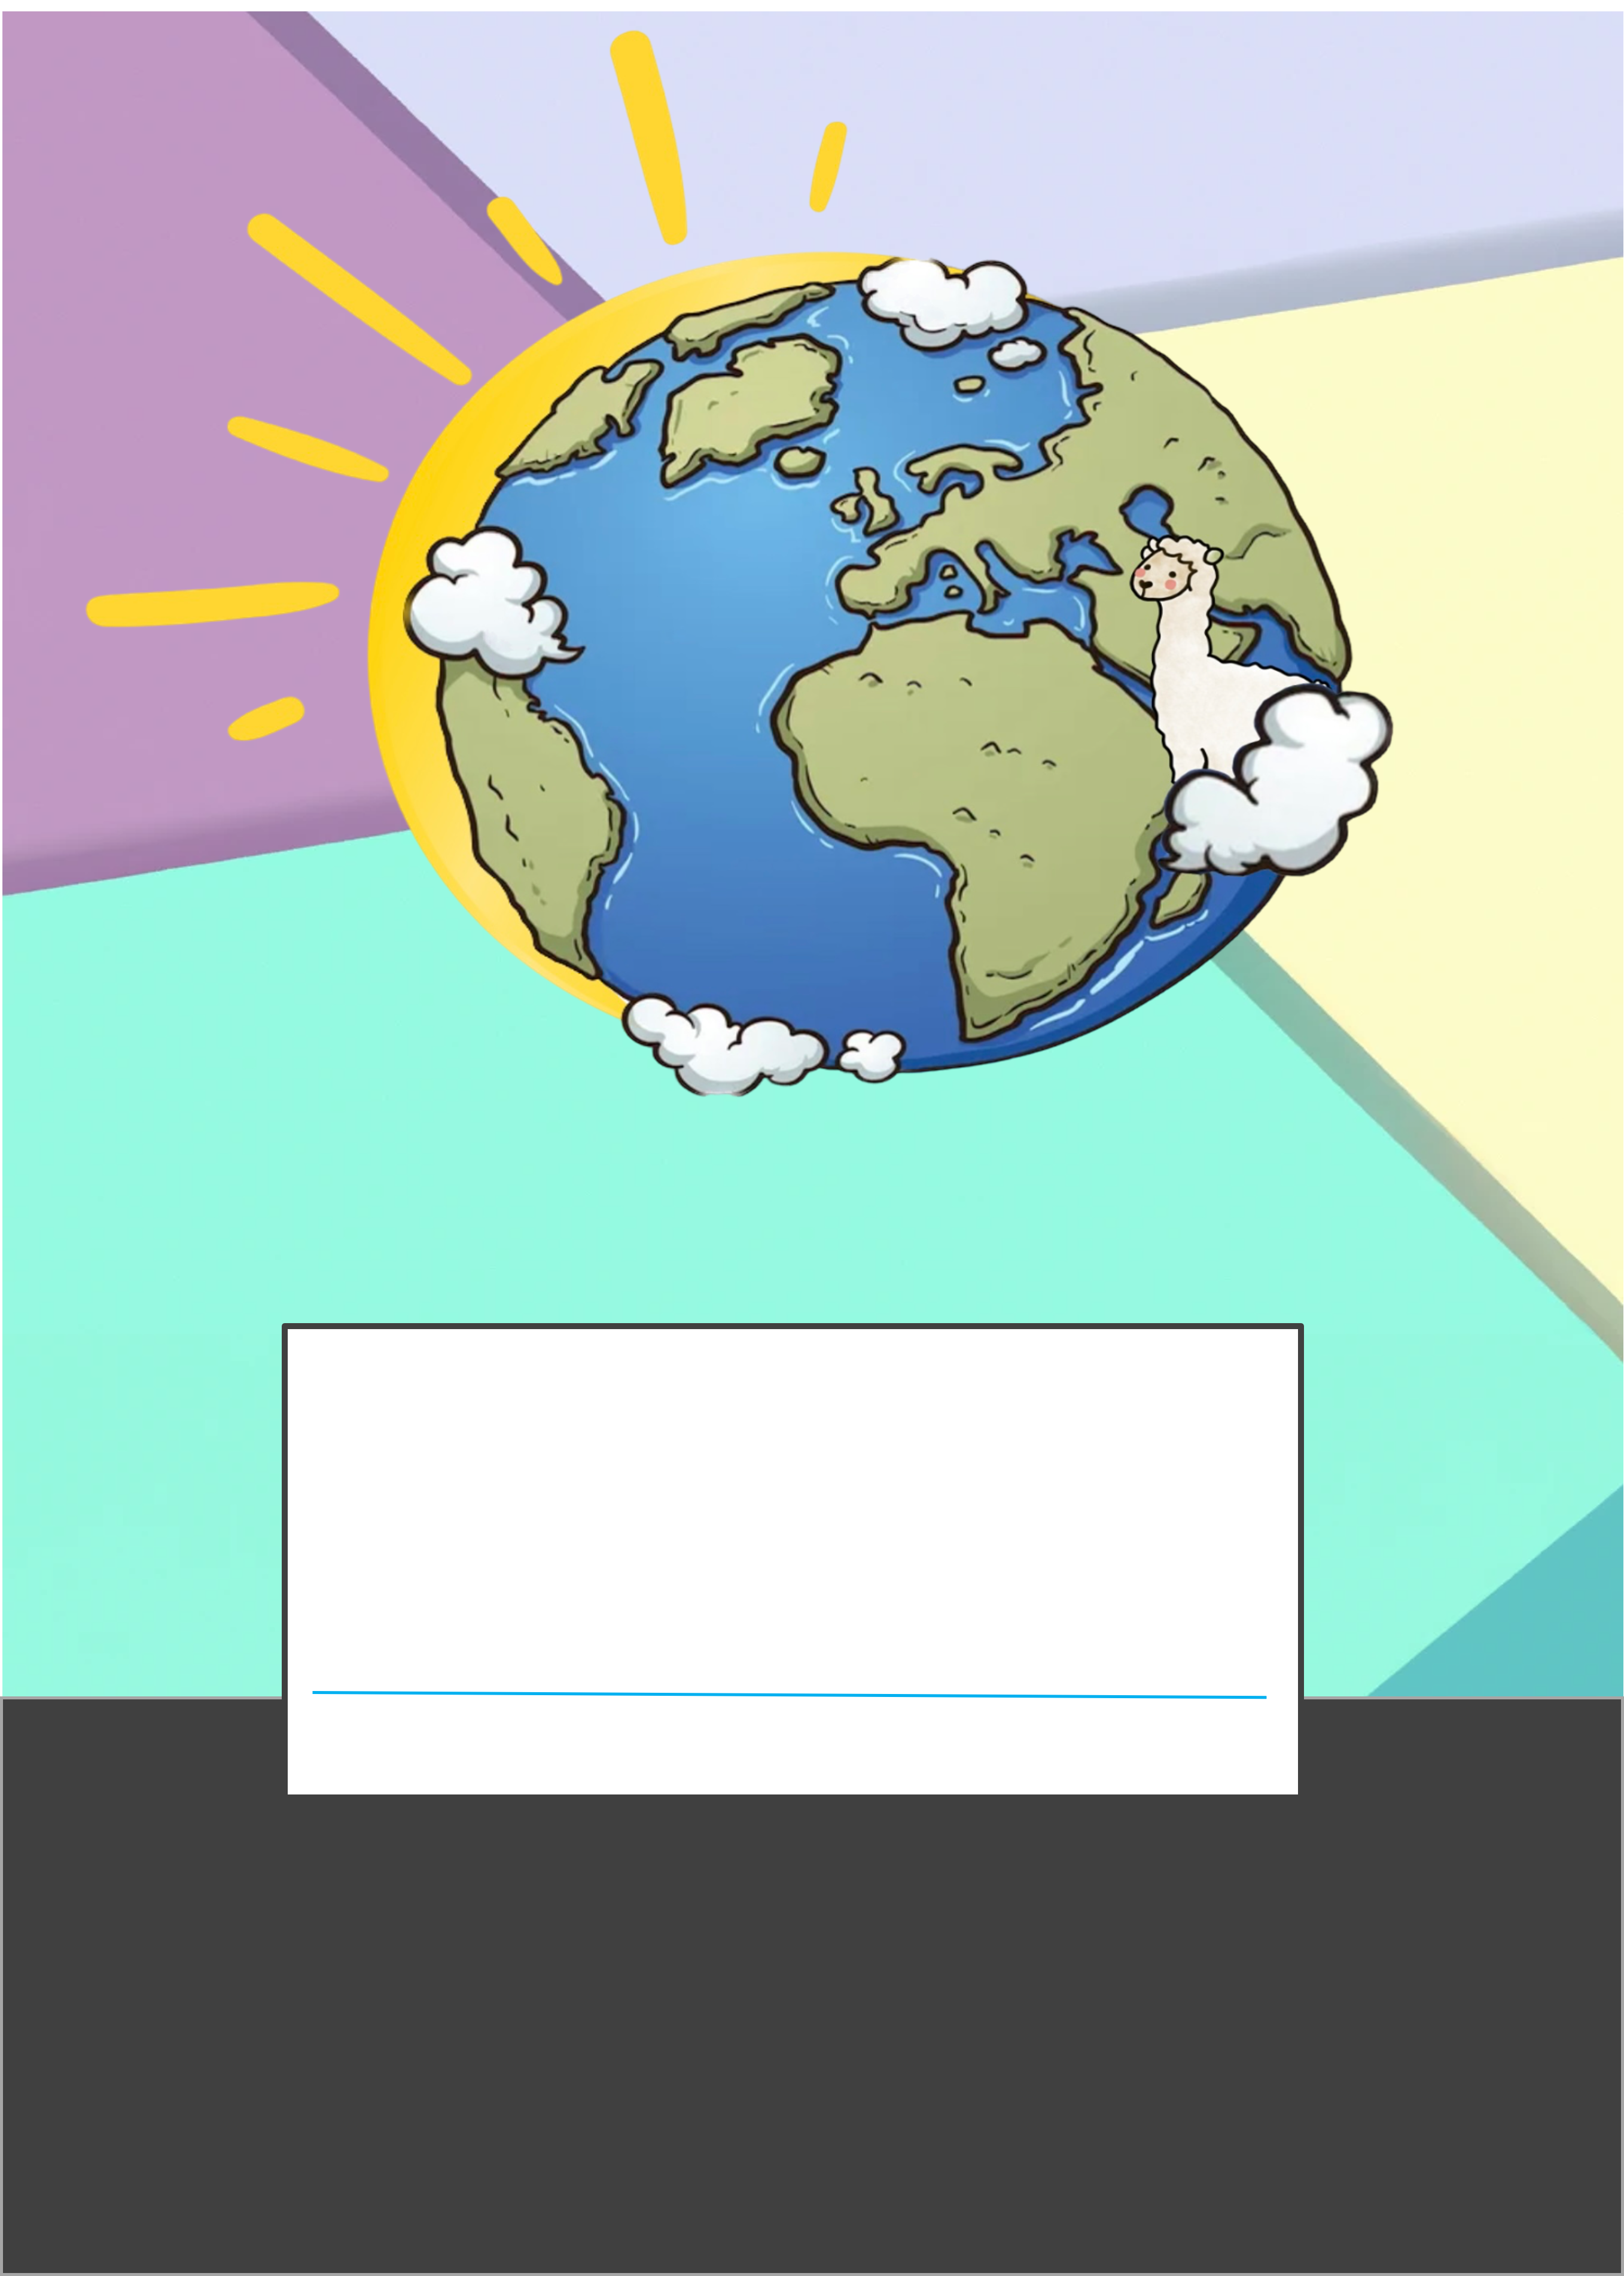
\includegraphics[width=\paperwidth,height=\paperheight,keepaspectratio]{../../img/firstpage_background.png}};
            \node[text=cyan, font=\fontsize{35}{50}\selectfont\bfseries] at ([xshift=-0.2cm,yshift=-4.5cm]current page.center) {Climate Monitoring};
            \node[text=cyan, font=\large] at ([xshift=-0.4cm,yshift=-7.5cm]current page.center) {\textit{Manuale Tecnico}};
            \node[text=white, font=\large] at ([xshift=-8.5cm,yshift=-9cm]current page.center) {Autori:};
            \node[text=white, font=\large] at ([xshift=-6.85cm,yshift=-10.5cm]current page.center) {Andrea Tettamanti 745387};
            \node[text=white, font=\large] at ([xshift=-7.28cm,yshift=-11.5cm]current page.center) {Luca Mascetti 752951};
            \node[text=white, font=\large] at ([xshift = 8cm, yshift = -9cm]current page.center) {Versione: 1.1};
            \node[text=white, font=\large] at ([xshift = 8cm, yshift = -10cm]current page.center) {Data: 07-02-2024};
        \end{tikzpicture}    }
}



\begin{document}



%frontespizio
\begin{titlepage}
    \null
\end{titlepage}

% Sovrapponi l'immagine al numero di pagina
\AddToShipoutPictureBG{
    \begin{tikzpicture}[overlay, remember picture]
        \node[inner sep=0pt, anchor=south] at ([xshift=-0.15cm,yshift=2.7cm]current page.south) {
\includegraphics[width=1.5cm,height=1.5cm]{../../img/number page.png}};
    \end{tikzpicture}
}

\clearpage
\NoBgThispage
\tableofcontents
\NoBgThispage
\listoffigures
\clearpage


\NoBgThispage
\section{Introduzione}
Benvenuti nell'applicazione \emph{Climate Monitoring}, software progettato per fornire accesso ai dati climatici 
provenienti dai centri di monitoraggio in tutta Italia. Questa applicazione è stata sviluppata con l'obiettivo di 
mettere a disposizione degli operatori ambientali e dei cittadini comuni dati accurati e rilevanti relativi alle 
condizioni climatiche della propria zona di interesse.

\section{Progettazione}

Il software è stato progettato seguendo un approccio client-server, in cui il server si occupa di ricevere i dati dai client e memorizzarli nel database, mentre i client possono richiedere i dati memorizzati al server.\\
Per la parte client, viene seguita l'architettura CMV (Controller-Model-View), in cui il controller e il view sono uniti nelle classi dell'interfaccia grafica, mentre il model è separato in un package a parte che 
permette l'uso dei metodi degli oggetti remoti presenti nel server. Questo viene fatto attraverso l'uso della tecnologia java RMI (Remote Method Invocation).
\NoBgThispage
\section{Struttura Generale dell'Applicazione}
L’applicazione è stata sviluppata seguendo l’architettura \texttt{MVC (Model-View-Controller)}, dove le parti View e Controller sono inglobati nella User Interface (UI).
Di conseguenza il codice sorgente del package \texttt{src} è suddiviso in due Macro-package: \texttt{Models} in cui sono presenti tutte le classi che gestiscono i dati,
mentre nel package \texttt{GUI} sono presenti le classi che gestiscono la UI e l’interazione tra i comandi fatti dall’utente e lo storage dei dati.
È presente anche un package, \texttt{utils}, che contiene classi di utilità usate nella maggior parte delle altre classi.


\begin{figure}[H]
    \centering
    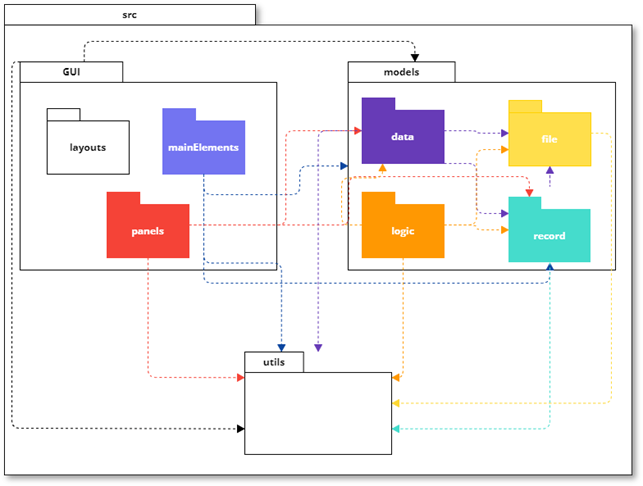
\includegraphics[width=0.7\textwidth]{../../img/package_structure.png}
    \caption{Struttura dei package dell'applicazione.}
\end{figure}
\section{Package shared}
In questa sezione verranno descritti il package \texttt{shared} e le classi che lo compongono.\\



\subsection{Package interfacesRMI}
In questa sezione verranno descritti il package \texttt{interfacesRMI} e le classi che lo compongono.\\

\begin{figure}[H]
    \centering
    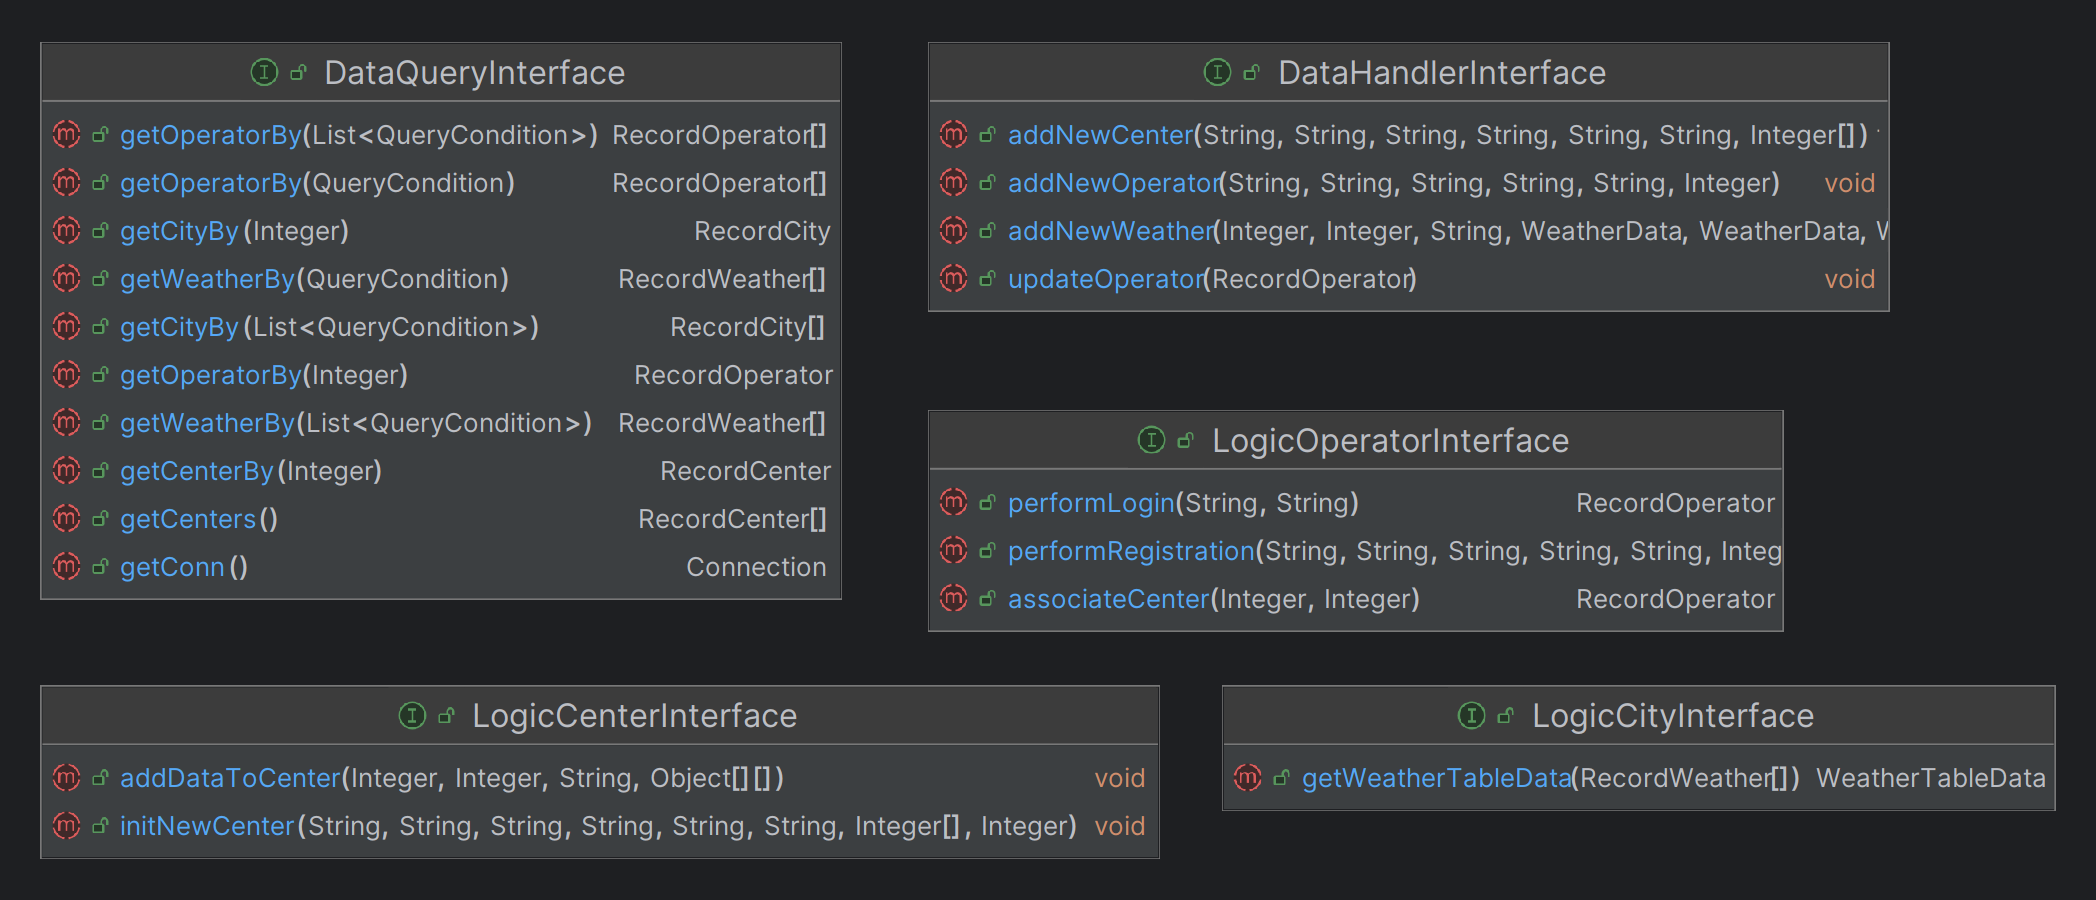
\includegraphics[scale = 0.2]{img/interfaceRMIPackage.png}
    \caption{UML delle classi del package interfacesRMI}
    \label{fig:InterfacesRMI}
\end{figure}

\subsubsection{DataHandlerInterface}
L'interfaccia \texttt{DataHandlerInterface} è un'interfaccia che permette di definire i metodi remoti che possono
essere invocati da un client per interagire con il server per la gestione dei dati.
Quest'interfaccia dev'essere implementata dalla classe \texttt{DataHandlerImp} la quale esegue i metodi dichiarati.
I metodi di tale interfaccia sono:
\begin{itemize}
    \item \texttt{void addNewOperator(String nameSurname, String taxCode, String email, String username, String password, Integer centerID)}
    \item \texttt{RecordCenter addNewCenter(String centerName, String streetName, String streetNumber, String CAP, String townName, String districtName, Integer[] cityIDs)}
    \item \texttt{void addNewWeather(Integer cityID, Integer centerID, String date, RecordWeather.WeatherData wind, RecordWeather.WeatherData humidity, RecordWeather.WeatherData pressure, RecordWeather.WeatherData temperature, RecordWeather.WeatherData precipitation, RecordWeather.WeatherData glacierElevation, RecordWeather.WeatherData glacierMass)}
    \item \texttt{void updateOperator(RecordOperator operator)}
\end{itemize}

\subsubsection{DataQueryInterface}
L'interfaccia \texttt{DataQueryInterface} è un'interfaccia che permette di definire i metodi remoti che possono
essere invocati da un client per interagire con il server per la gestione dei dati.
Quest'interfaccia dev'essere implementata dalla classe \texttt{DataQueryImp} la quale esegue i metodi dichiarati.
I metodi di tale interfaccia sono:
\begin{itemize}
    \item \texttt{RecordCity getCityBy(Integer ID)}
    \item \texttt{RecordCity[] getCityBy(List<QueryCondition> conditions)}
    \item \texttt{RecordOperator getOperatorBy(Integer ID)}
    \item \texttt{RecordOperator[] getOperatorBy(QueryCondition condition)}
    \item \texttt{RecordOperator[] getOperatorBy(List<QueryCondition> conditions)}
    \item \texttt{RecordCenter getCenterBy(Integer ID)}
    \item \texttt{RecordCenter[] getCenters()}
    \item \texttt{RecordWeather[] getWeatherBy(QueryCondition condition)}
    \item \texttt{RecordWeather[] getWeatherBy(List<QueryCondition> conditions)}
    \item \texttt{Connection getConn()}
\end{itemize}

\subsubsection{LogicCenterInterface}
L'interfaccia \texttt{LogicCenterInterface} è un'interfaccia che permette di definire i metodi remoti che possono
essere invocati da un client per interagire con il server per la gestione dei centri di monitoraggio.
Quest'interfaccia dev'essere implementata dalla classe \texttt{LogicCenterImp} la quale esegue i metodi dichiarati.
I metodi di tale interfaccia sono:
\begin{itemize}
    \item \texttt{void initNewCenter(String centerName, String streetName, String streetNumber, String CAP, String townName, String districtName, Integer[] cityIDs, Integer operatorID)}
    \item \texttt{void addDataToCenter(Integer cityID, Integer operatorID, String date, Object[][] tableData)}
\end{itemize}

\subsubsection{LogicCityInterface}
L'interfaccia \texttt{LogicCityInterface} è utilizzata per esporre i metodi che permettono di ottenere i dati relativi alle città, in particolare i dati metereologici.
Quest'interfaccia dev'essere implementata dalla classe \texttt{LogicCityImp} la quale esegue i metodi dichiarati.
L'unico metodo di tale classe è:
\begin{itemize}
    \item \texttt{LogicCityImp.WeatherTableData getWeatherTableData(RecordWeather[] weatherRecords)}
\end{itemize}

\subsubsection{LogicOperatorInterface}
L'interfaccia \texttt{LogicOperatorInterface} è un'interfaccia che permette di definire i metodi remoti che possono essere invocati da un client per interagire con il server per la gestione della logica di business degli operatori.
Quest'interfaccia dev'essere implementata dalla classe \texttt{LogicOperatorImp} la quale esegue i metodi dichiarati.
I metodi di tale interfaccia sono:
\begin{itemize}
    \item \texttt{RecordOperator performLogin(String username, String password)}
    \item \texttt{void performRegistration(String nameSurname, String taxCode, String email, String username, String password, Integer centerID)}
    \item \texttt{RecordOperator associateCenter(Integer operatorID, Integer centerID)}
\end{itemize}

\subsection{Package record}
In questa sezione verranno descritti il package \texttt{record} e le classi che lo compongono.\\

\begin{figure}[H]
    \centering
    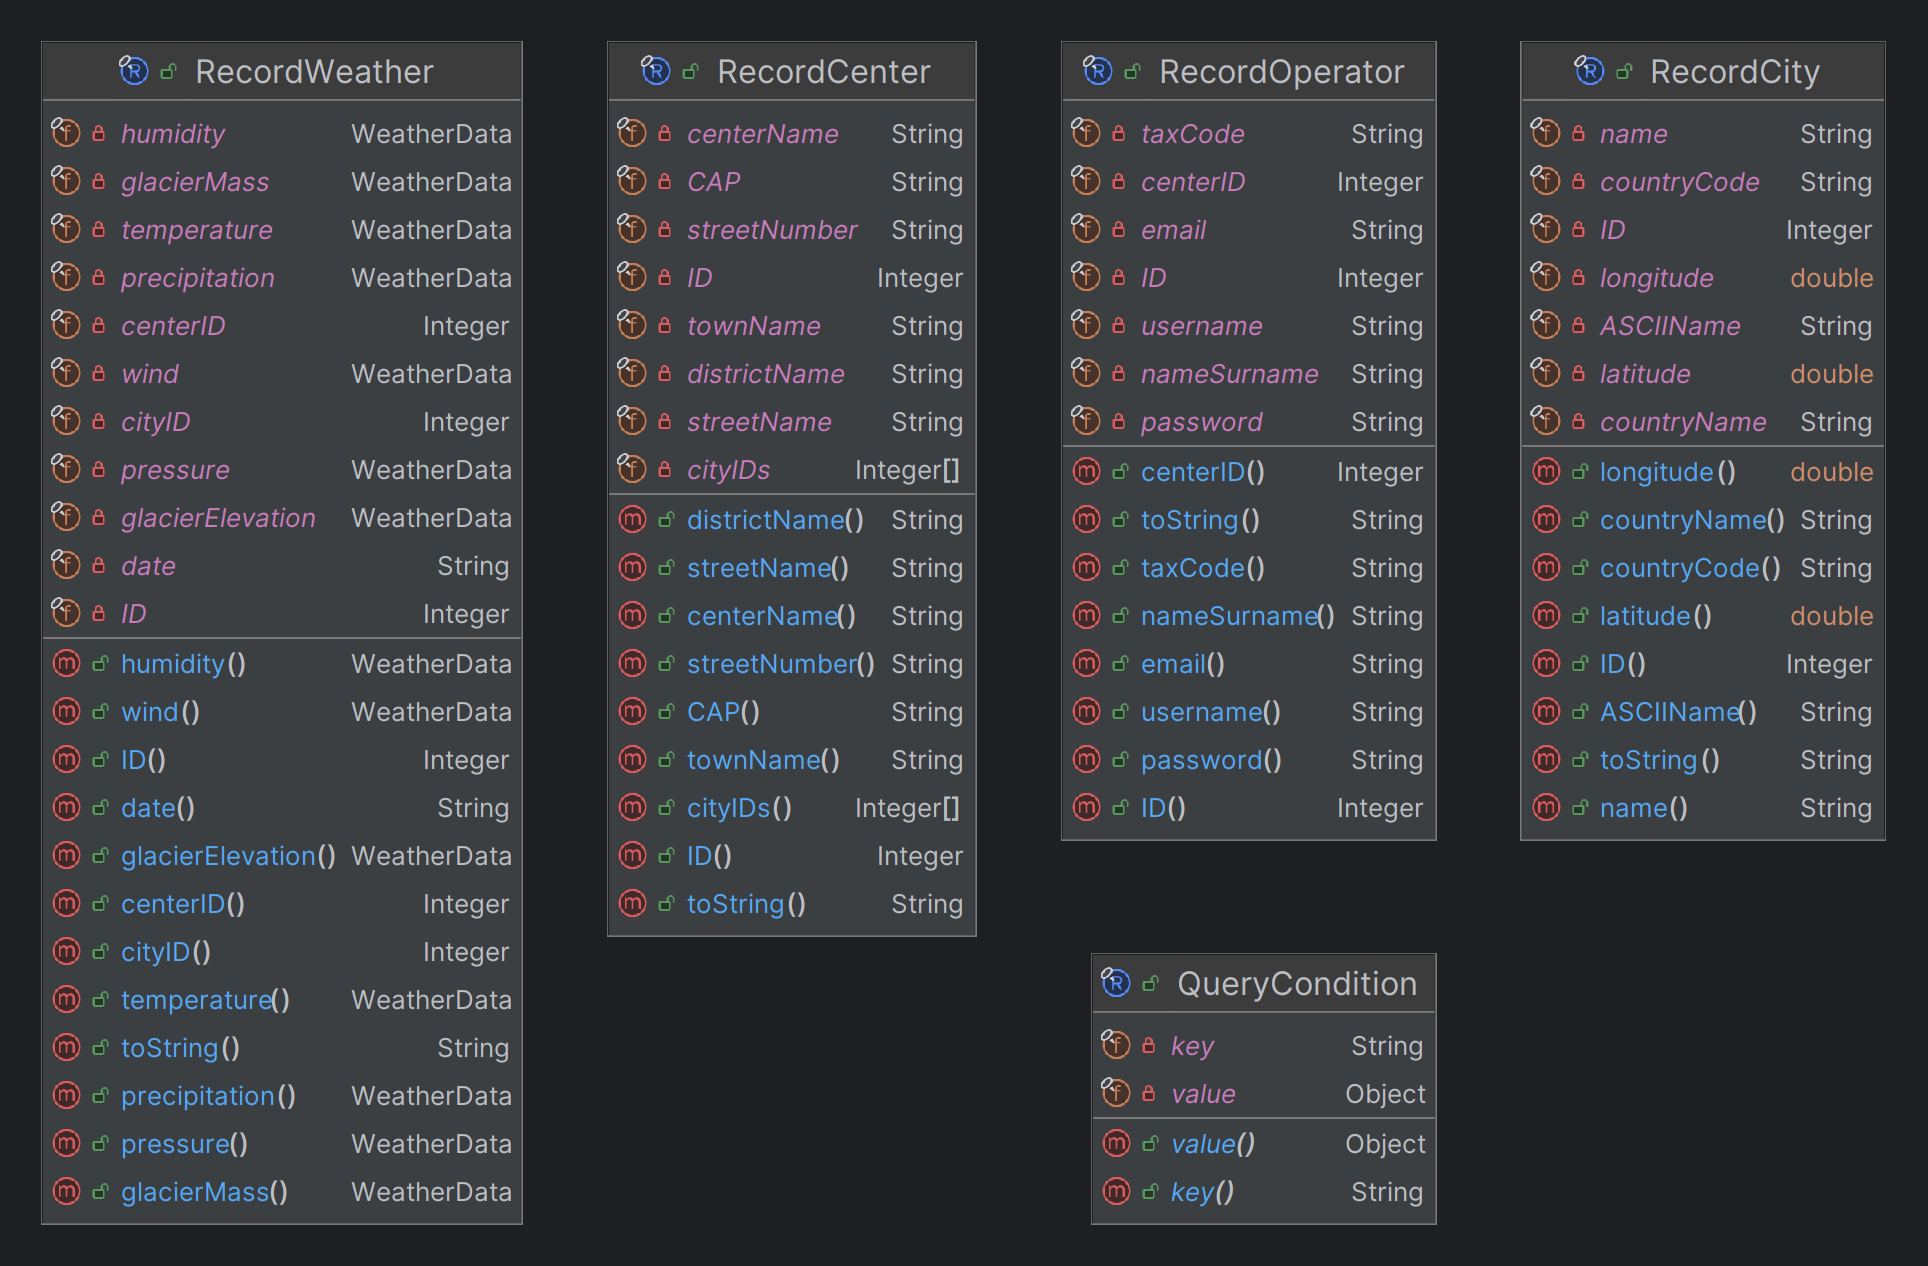
\includegraphics[scale = 0.2]{img/recordPackage.png}
    \caption{UML delle classi del package record}
    \label{fig:Record}
\end{figure}
\subsubsection{QueryCondition}
La classe \texttt{QueryCondition} rappresenta una condizione di query.\\
Viene utilizzata per definire una condizione di ricerca per i record presenti nel database.

\subsubsection{RecordCenter}
La classe \texttt{RecordCenter} rappresenta un centro di monitoraggio e contiene informazioni come il nome del centro, il nome della via, il numero civico, il CAP, il nome del comune, la sigla della provincia e una lista di ID delle città associate.
Questa classe è definita come un record, il che significa che è immutabile una volta creata.
I metodi di tale classe sono:
\begin{itemize}
    \item \texttt{public String toString()}
    \item \texttt{public Integer ID()}
    \item \texttt{public String centerName()}
    \item \texttt{public String streetName()}
    \item \texttt{public String streetNumber()}
    \item \texttt{public String CAP()}
    \item \texttt{public String townName()}
    \item \texttt{public String districtName()}
    \item \texttt{public String cityIDs()}
\end{itemize}

\subsubsection{RecordCity}
La classe \texttt{RecordCity} rappresenta una città e contiene informazioni come l'ID della città, il nome, il nome ASCII, il codice del paese, il nome del paese, la latitudine e la longitudine geografica.
Questa classe è definita come un record, il che significa che è immutabile una volta creata.
I metodi di tale classe sono:
\begin{itemize}
    \item \texttt{public String toString()}
    \item \texttt{public Integer ID()}
    \item \texttt{public String name()}
    \item \texttt{public String ASCIIname()}
    \item \texttt{public String countryCode()}
    \item \texttt{public String countryName()}
    \item \texttt{public double latitude()}
    \item \texttt{public double longitude()}
\end{itemize}

\subsubsection{RecordOperator}
La classe \texttt{RecordOperator} rappresenta un operatore e contiene informazioni come l'ID, il nome e cognome, il codice fiscale, l'email, il nome utente, la password e l'ID del centro di competenza (se assegnato).
Questa classe è definita come un record, il che significa che è immutabile una volta creata.
I metodi di tale classe sono:
\begin{itemize}
    \item \texttt{public String toString()}
    \item \texttt{public Integer ID()}
    \item \texttt{public String nameSurname()}
    \item \texttt{public String taxCode()}
    \item \texttt{public String email()}
    \item \texttt{public String username()}
    \item \texttt{public String password()}
    \item \texttt{public Integer centerID()}
\end{itemize}

\subsubsection{RecordWeather}
La classe \texttt{RecordWeather} rappresenta dati meteorologici registrati in una determinata data per una città e un centro specifici.
Questa classe contiene informazioni come l'ID, l'ID della città, l'ID del centro, la data e vari dati meteorologici come il vento, l'umidità, la pressione, la temperatura, la precipitazione, l'elevazione del ghiacciaio e la massa del ghiacciaio.
Questa classe è definita come un record, il che significa che è immutabile una volta creata.
I metodi di tale classe sono:
\begin{itemize}
    \item \texttt{public String toString()}
    \item \texttt{public Integer ID()}
    \item \texttt{public Integer cityID()}
    \item \texttt{public Integer centerID()}
    \item \texttt{public String date()}
    \item \texttt{public WeatherData wind()}
    \item \texttt{public WeatherData humidity()}
    \item \texttt{public WeatherData pressure()}
    \item \texttt{public WeatherData temperature()}
    \item \texttt{public WeatherData precipitation()}
    \item \texttt{public WeatherData glacierElevation()}
    \item \texttt{public WeatherData glacierMass()}
    \item \texttt{public Integer score()}
    \item \texttt{public String comment()}
\end{itemize}

\subsection{Package utils}
In questa sezione verranno descritti il package \texttt{utils} e le classi che lo compongono.\\

\begin{figure}[H]
    \centering
    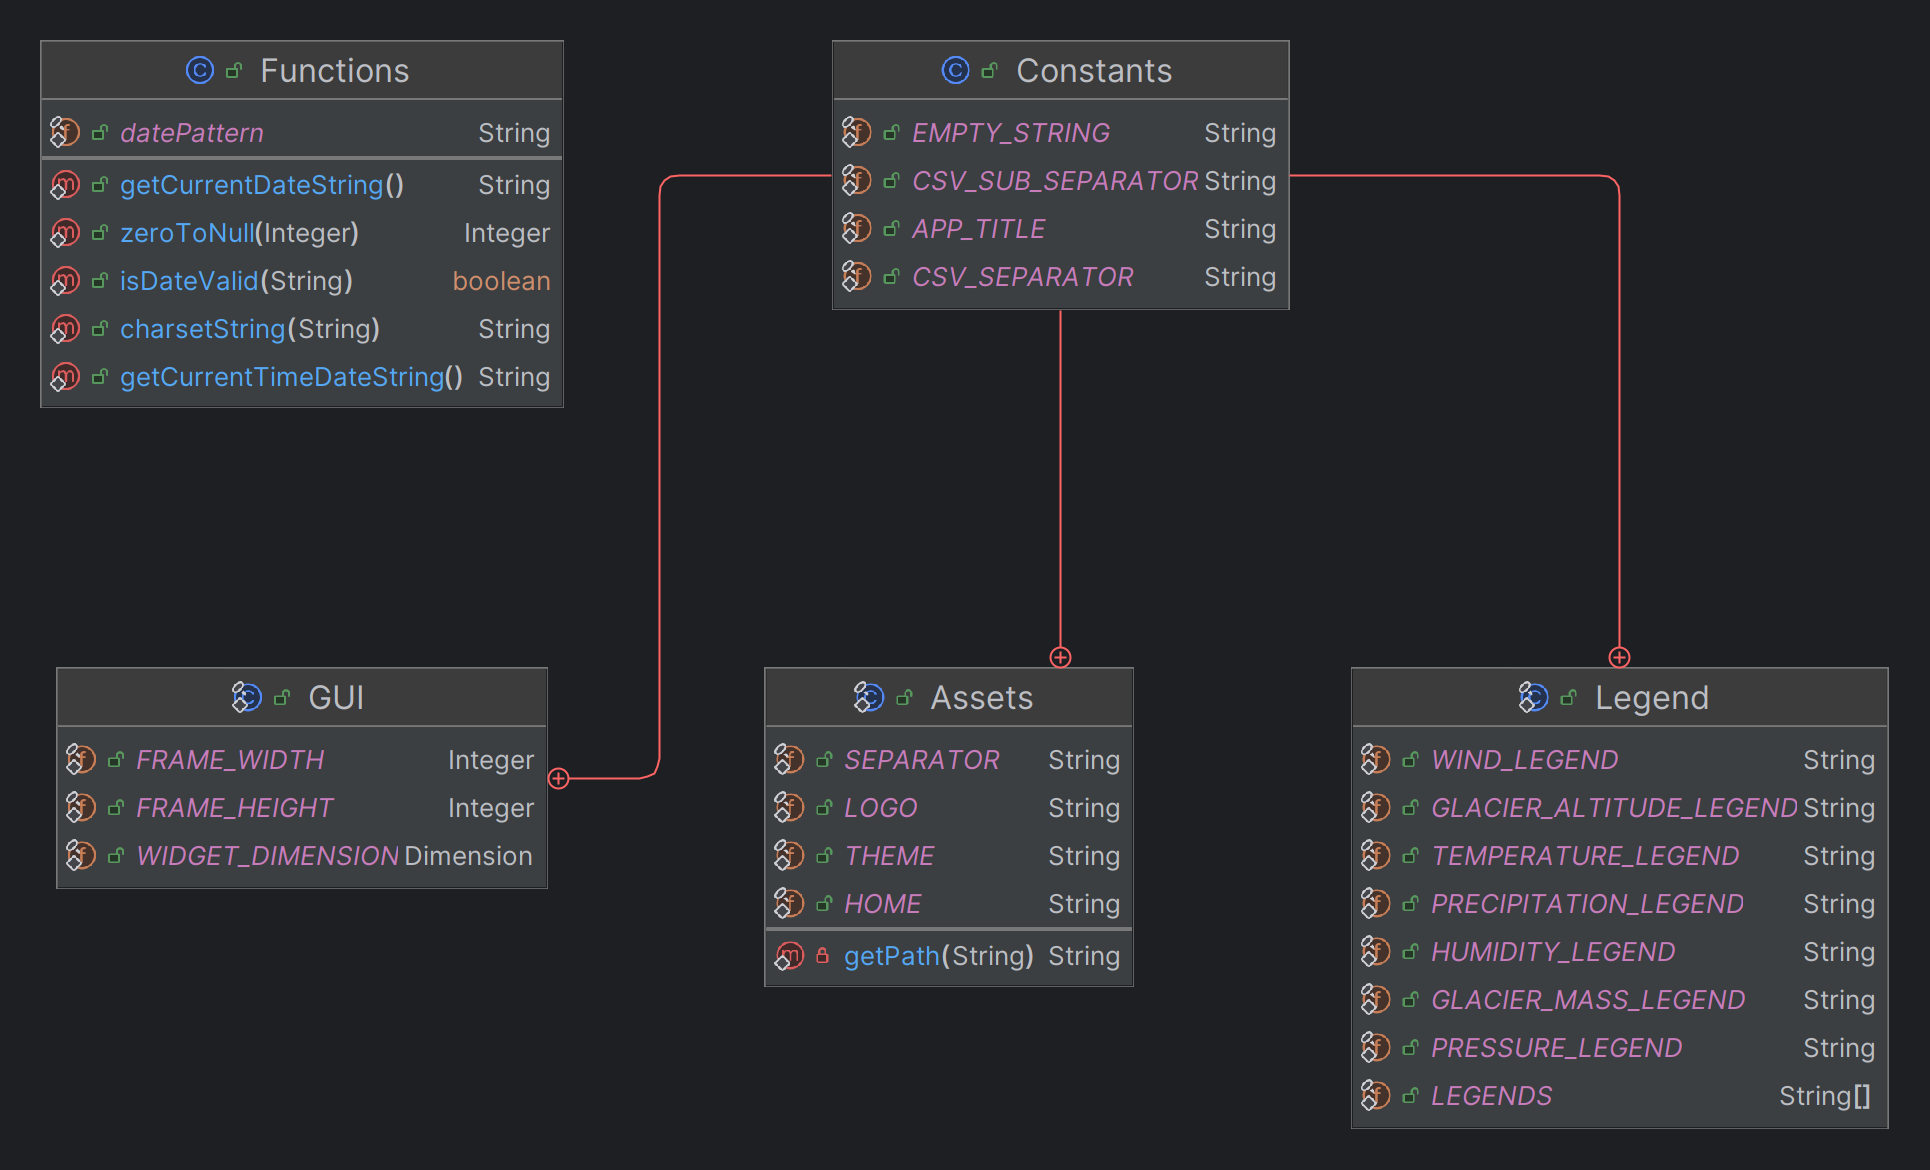
\includegraphics[scale = 0.2]{img/utils_1.png}
    \caption{UML delle classi Functions e Constants}
    \label{fig:Utils1}    
\end{figure}

\begin{figure}[H]
    \centering
    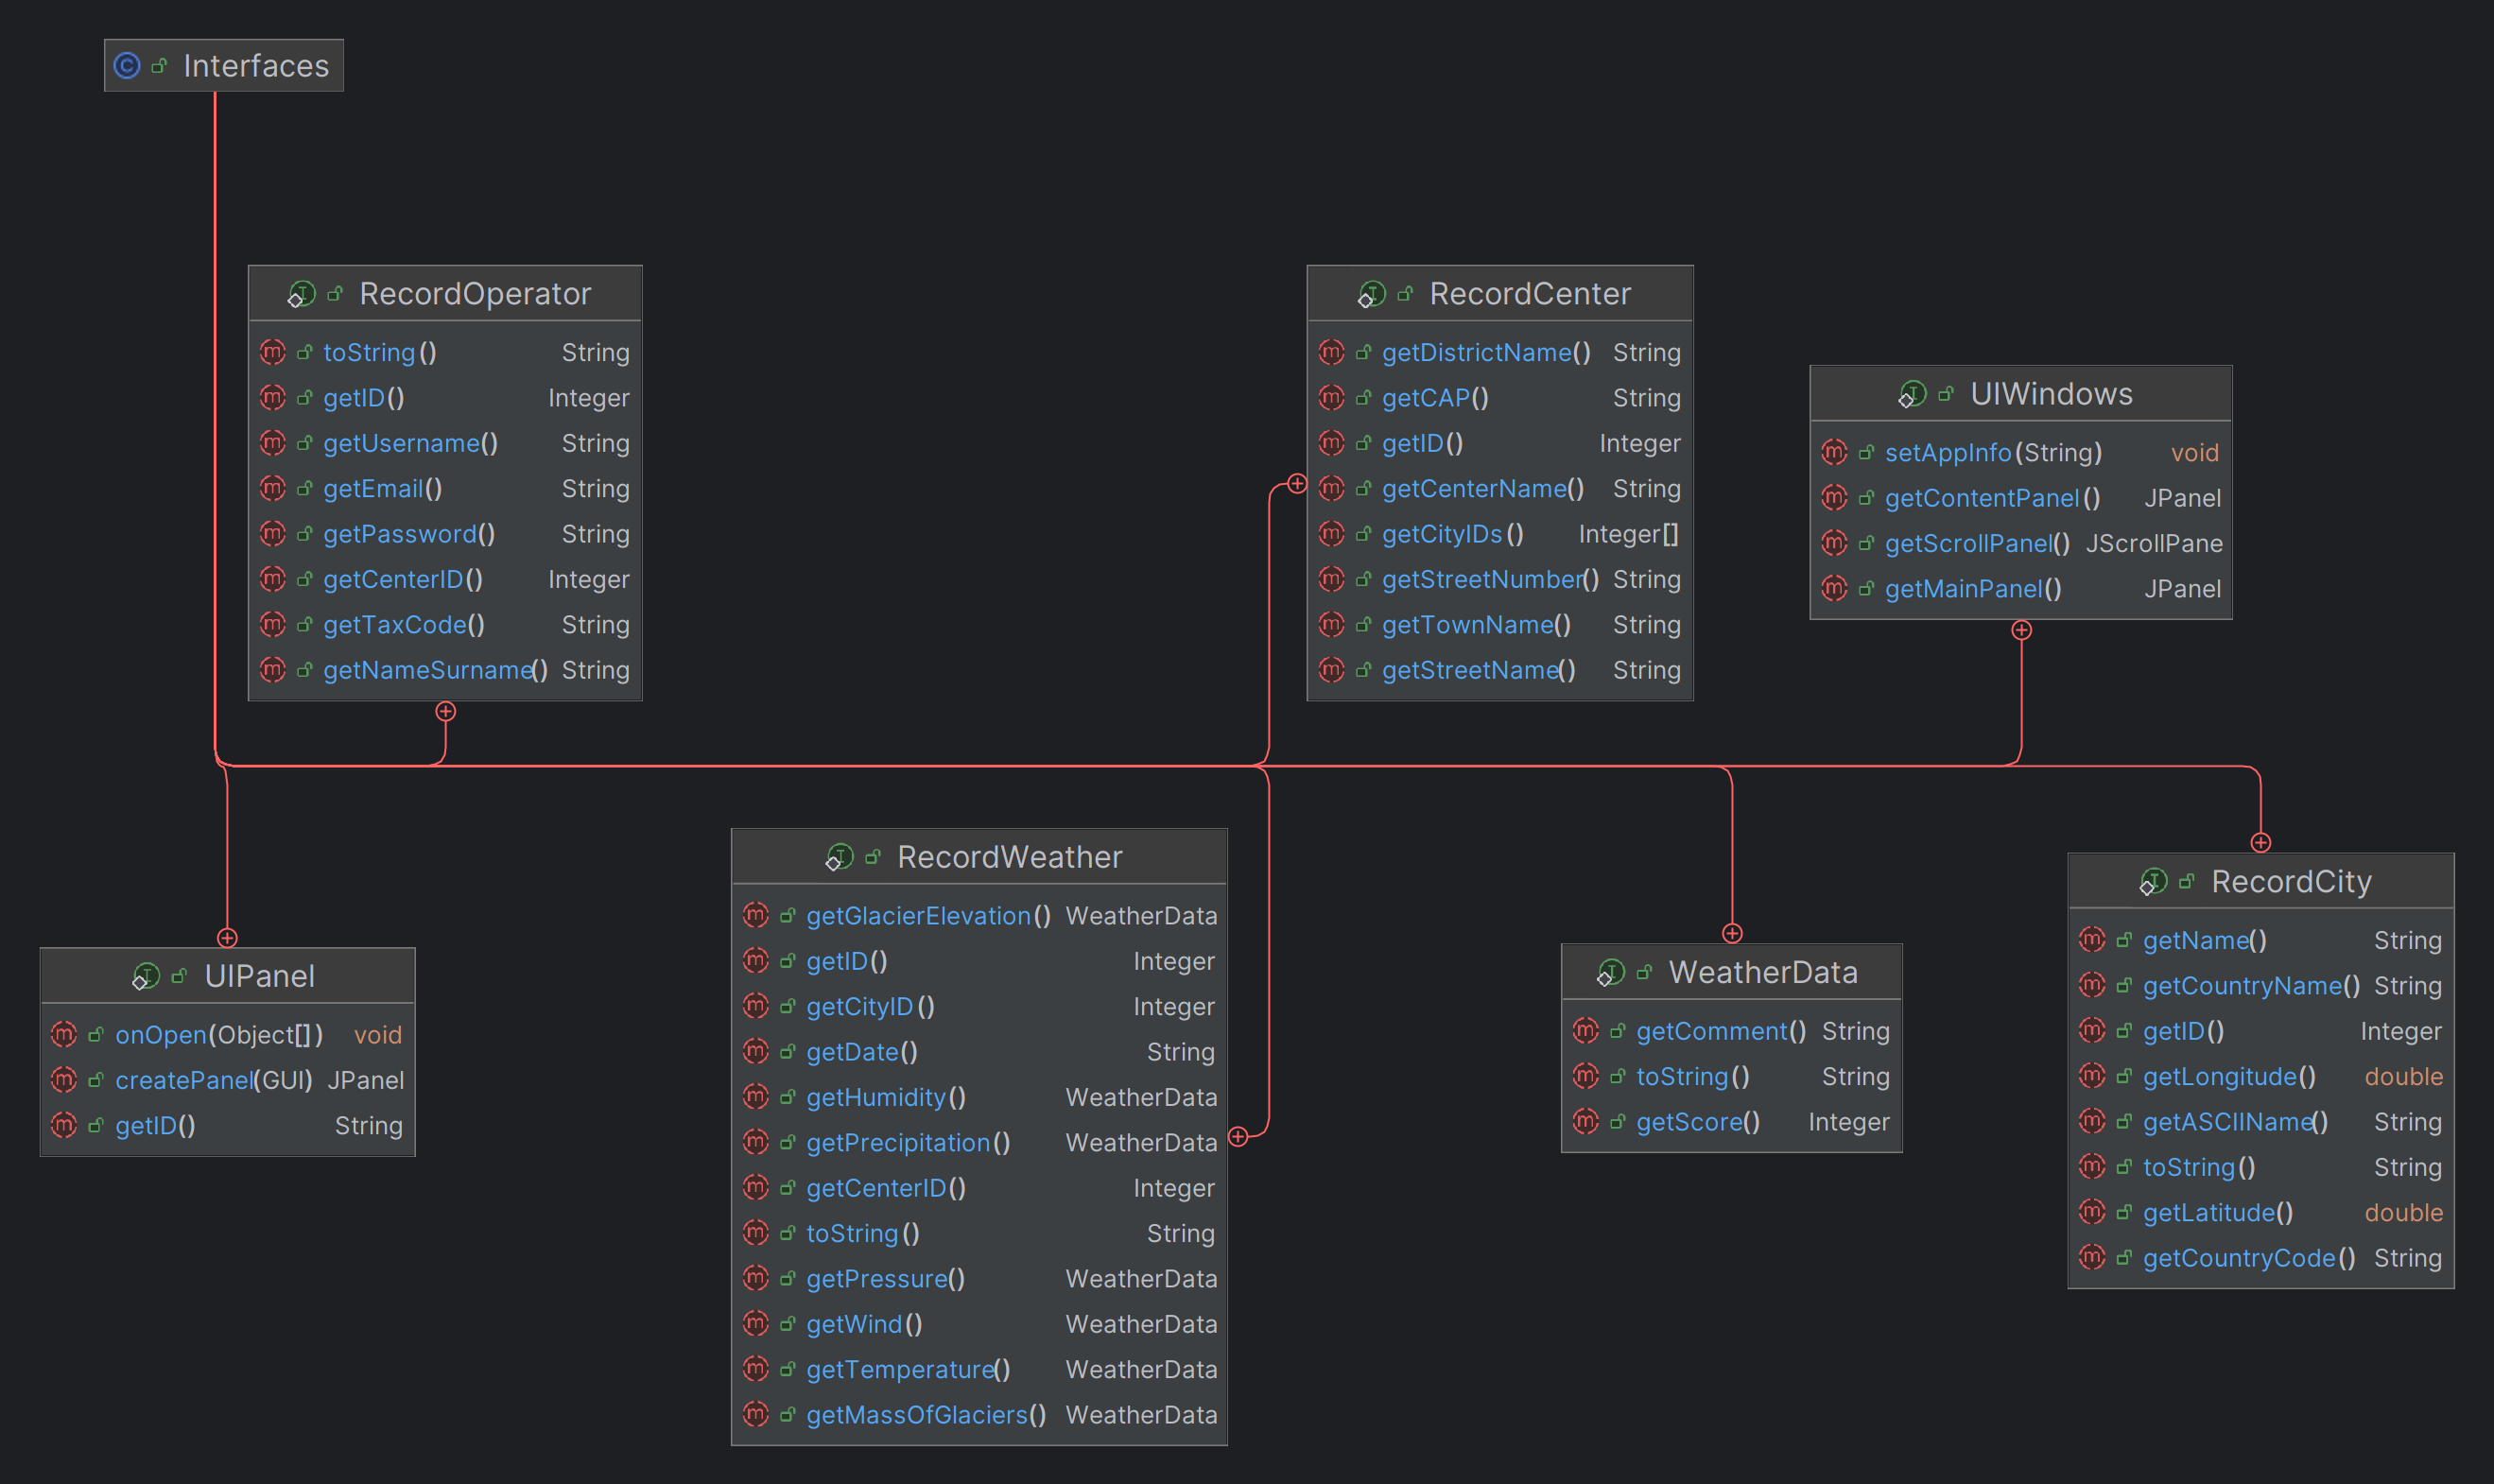
\includegraphics[scale = 0.1]{img/utils_2.png}
    \caption{UML delle classi Interfaces}
    \label{fig:Utils2}    
\end{figure}

\subsubsection{Constants}
La classe \texttt{Constants} fornisce una serie di costanti e definizioni utilizzate nell'applicazione.
Queste costanti includono separatori CSV, titolo dell'applicazione, indici di dati, percorsi dei file, dimensioni GUI predefinite e dati predefiniti.
La classe è progettata per memorizzare costanti utilizzate in tutto il codice e semplificare eventuali modifiche future.

\subsubsection{Functions}
La classe \texttt{Functions} fornisce una serie di funzioni di utilità per la gestione delle date e degli orari.
Queste funzioni includono la generazione della data corrente, la validazione delle date e la generazione della data e dell'orario correnti.
I metodi di tale classe sono:
\begin{itemize}
    \item \texttt{public static String getCurrentDateString()}: restituisce una stringa rappresentante la data corrente nel formato \textbf{yyyy-MM-dd}.
    \item \texttt{public static boolean isDateValid(String dateString)}: verifica se una stringa rappresentante una data è valida e non successiva alla data corrente.
    \item \texttt{public static String getCurrentTimeDateString()}: restituisce una stringa rappresentante la data e l'orario correnti nel formato \textbf{yyyy-MM-dd HH:mm:ss}.
    \item \texttt{public static String charsetString(String string)}: converte una stringa in un formato compatibile con il charset UTF-8.
    \item \texttt{public static Integer zeroToNull(Integer value)}: converte un valore 0 in un valore nullo.
\end{itemize}

\subsubsection{Interfaces}
L'interfaccia \texttt{Interfaces} definisce una serie di interfacce e contratti che rappresentano diversi aspetti ed entità all'interno del sistema.
Queste interfacce definiscono le proprietà e i metodi che devono essere implementati da classi specifiche per fornire funzionalità legate a città, operatori, centri, dati meteorologici, finestre UI e pannelli UI.
Per le interfacce dei record i metodi sono i getter degli attributi.
Invece per l'interfaccia di UI Windows i metodi sono:
\begin{itemize}
    \item \texttt{JPanel getMainPanel()}
    \item \texttt{JScrollPane getScrollPanel()}
    \item \texttt{JPanel getContentPanel()}
    \item \texttt{void setAppInfo(String text)}
\end{itemize}
Infine per l'interfaccia di UI Panel i metodi sono:
\begin{itemize}
    \item \texttt{JPanel createPanel(GUI gui)}
    \item \texttt{void onOpen(Object[] args)}
    \item \texttt{String getID()}
\end{itemize}


\section{Package Server}
In questa sezione verranno descritti il package \texttt{server} e le classi che lo compongono.\\

\begin{figure}[H]
    \centering
    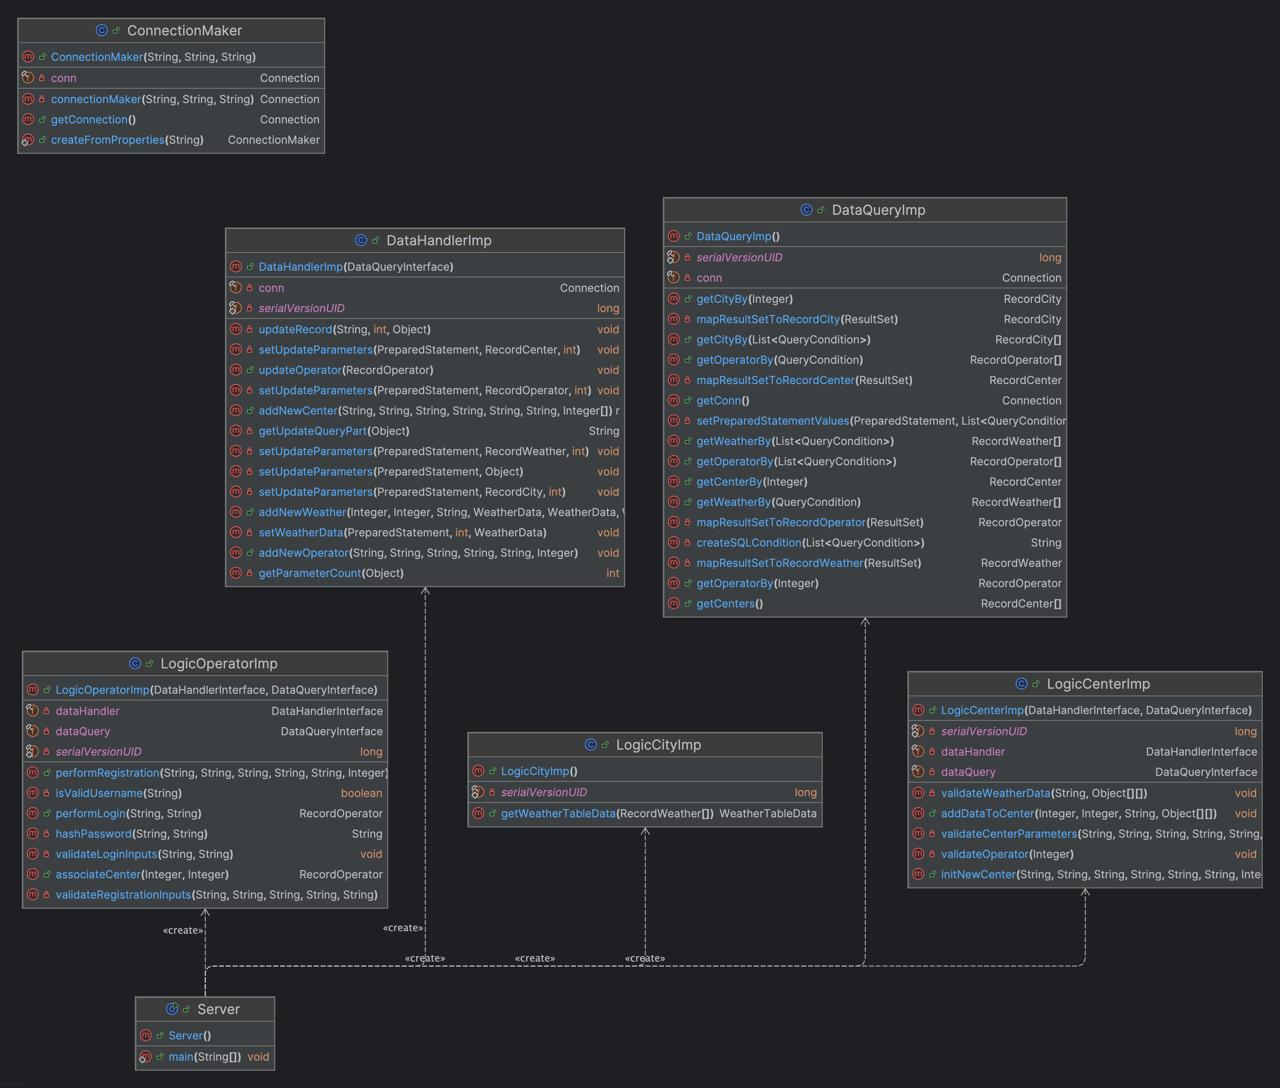
\includegraphics[width=0.9\textwidth]{img/serverClassDiagram.jpg}
    \caption{UML del package Server}
    \label{fig:Server}
\end{figure}

\subsection{Server}
La classe \texttt{Server} è progettata per avviare il registro RMI e pubblicare le implementazioni delle interfacce remote.\\
Queste implementazioni sono accessibili ai client remoti, che possoo invocare metodi per interrogare, gestire e manipolare i dati relativi alle operazioni dell'applicazione.\\
In sisntesi, \texttt{Server} svolge le seguenti operazioni principali:
\begin{itemize}
    \item \textbf{Creazione e Configurazione del Registro RMI}: avvia un registro RMI sulla porta specificata (di default, la porta 1099) utilizzando il metodo\\
          \texttt{LocateRegistry.createRegistry(int port)}. Questo registro permette ai client remoti di trovare e invocare i metodi delle interfacce registrate.
    \item \textbf{Inizializzazione delle Implementazioni RMI}: la classe crea istanze delle implementazioni delle interfacce remote che gestiscono diverse logiche di business.
          Queste implementazioni sono
          \begin{itemize}
              \item \texttt{DataQueryImp}
              \item \texttt{DataHandlerImp}
              \item \texttt{LogicOperatorImp}
              \item \texttt{LogicCenterImp}
              \item \texttt{LogicCityImp}
          \end{itemize}
    \item \textbf{Registrazione delle Implementazioni nel Registro RMI}: ogni implementazione viene registrata nel registro RMI con un nome specifico utilizzando il metodo
          \texttt{rebind(String name, Remote obj)}. Questo passaggio rende i metodi delle interfacce remote accessibili ai client remoti trmite il nome associato.
\end{itemize}

\subsection{ConnectionMaker}
La classe \texttt{ConnectionMaker} è progettata per gestire la connessione al database, utilizzando sia parametr5i espliciti che file di configurazione.\\
La gestione della connessione viene effettuata tramite l'oggetto \texttt{Connection}, che rappresenta un collegamento la database, permettendo l'esecuzione di query e altre operazioni di manipolazione dei dati.\\
\\
I metodi pubblici sono:
\begin{itemize}
    \item \texttt{createFromProperties(String filepath)}:
          questo metodo statico consente di creare un'istanza di \texttt{ConnectionMaker} utilizzando un file di properties. Il file specificato deve contenere le chiavi \texttt{db.url}, \texttt{db.username} e \texttt{db.password},
          che vengono lette e utilizzate per stabilire la connessione al databse.
          Se il file non viene trovato o si verifica un errore durante la lettura, viene lanciata un'eccezione.
    \item \texttt{getConnection()}:
          questo metodo pubblico restituisce l'oggetto \texttt{Connection} gestito da \texttt{ConnectionMaker}. Questo permette ad altre classi del sistema di accedere alla connessione per eseguire operazioni di query, aggiornamento o altre interazioni con il database.
\end{itemize}
I metodi privati sono:
\begin{itemize}
    \item \texttt{connectionMaker(String url, String username, String password)}:
          questo metodo privato è responsabile della creazione effettiva della connessione al databse. Utilizza l'URL, il nome utene e la password per creare un oggetto \texttt{Connection} tramite il \texttt{DriverManager} di JDBC. Il metodo configura anche un oggetto \texttt{Properties} pre gestire le credenziali di accesso.
\end{itemize}




\subsection{Package ImplementationRMI}
Il package \texttt{ImplementationRMI} contiene le classi che implementano le interfacce remote definite nel package \texttt{InterfacesRMI} e che gestiscono le logiche di business dell'applicazione.\\


\subsubsection{DataHandlerImp}
La classe \texttt{DataHandlerImp} implementa l'interfaccia \texttt{DataHandlerInterface} e si occupa di gestire operazioni aggiunte e aggiornamento dei record nel database.
Questa classe utilizza JDBC per interagire con il database e fornisce metodi per gestire i record relativi agli operatori, ai centri di monitoraggio e ai dati climatici.\\
\\
I metodi pubblici sono:
\begin{itemize}
    \item \texttt{addNewOperator(String nameSurname, String taxcode, String email, String username, String password, Integer centerID)}:
          aggiunge un nuovo operatore al databse. Prima di inserire i dati, viene effettuato un controllo per assicurarsi che l'utente non esista già.
          Lancia eccezioni \texttt{SQLException, RemoteException, IllegalArgumentException} in caso di errori.
    \item \texttt{addNewCenter(String centerName, String streetName, String streetNumber, String CAP, String townName, String districName, Integer[] cityIDs)}:
          aggiunge un nuovo centro di monitoraggio al database. Prima di inserire i dati, viene effettuato un controllo per evitare duplicati. Restituisce un oggetto \texttt{RecordCenter} che rappresenta il centro appena inserito.
          Lancia eccezioni \texttt{SQLException, RemoteException, IllegalArgumentException} in caso di errori.
    \item \texttt{addNewWeather(Integer cityID, Integer centerID, String date, RecordWeather.WeatherData wind, RecordWeather.WeatherData humidity, RecordWeather.WeatherData pressure, RecordWeather.WeatherData temperature, RecordWeather.WeatherData precipitation, RecordWeather.WeatherData glacierElevation, RecordWeather.WeatherData glacierMass)}:
          aggiunge nuovi dati climatici al database associati a una spoecifica città e centro di monitoraggio. Gestisce il formato della data e l'inerimento dei dati climatici in modo dettagliato.
          Lancia eccezioni \texttt{SQLException, RemoteException} in caso di errori.
    \item \texttt{updateOperator(RecordOperator operator)}:
          aggiorna le informazioni di un operatore nel database. Utilizza un metodo interno \texttt{updateRecord} per eseguire l'operazione.
          Lancia eccezioni \texttt{SQLException, RemoteException} in caso di errori.
\end{itemize}
I metodi privati sono:
\begin{itemize}
    \item \texttt{updateRecord(String tableName, int ID, Object record)}:
          esegue l'aggiornamento di un record specifico nel database sulla base del tipo di record e dell'ID fornito.
    \item \texttt{getUpdateQueryPart(Object object)}:
          genera dinamicamente la stringa SQL necessaria per l'aggiornamento di un record di base al tipo di oggetto (ad esempio, \texttt{RecordOperator} o \texttt{RecordCenter}).
    \item \texttt{setUpdateParameters(PreparedStatement stmt, Object object)}:
          imposta i parametri di un oggetto \texttt{PreparedStatement} per l'aggiornamento di un record.
    \item \texttt{setWeatherData(PreparedStatement stmt, int index, RecordWeather.WeatherData data)}:
          imposta i dati climatici (score e commenti) all'interno del \texttt{PreparedStatement} per l'inserimento o l'aggiornamento.
    \item \texttt{getParameterCount(Object record)}:
          restituisce il numero di parametri per un determianto tipo di record, necessario per costruire la query SQL.
\end{itemize}

\subsubsection{DataQueryImp}
La classe \texttt{DataQueryImp} implementa l'interfaccia \texttt{DataQueryInterface} e consente di eseguire query sul database per ottenere informazioni relative a città, operatori, centri di monitoraggioe e dati climatici.\\
\\
I metodi pubblici sono:
\begin{itemize}
    \item \texttt{getCityBy(Integer ID)}: restituisce un oggetto \texttt{RecordCity} contenente le informazioni di una città basandosi sul suo ID.
    \item \texttt{getOperatorBy(Integer ID)}: restituisce un oggetto \texttt{RecordOperator} contenente le informazioni di un operatore basandosi sul suo ID.
    \item \texttt{getCenterBy(Integer ID)}: restituisce un oggetto \texttt{RecordCenter} contenente le informazioni di un centro di monitoraggio basandosi sul suo ID.
    \item \texttt{getCityBy(List<QueryCondition> conditions)}: restituisce un array di oggetti \texttt{RecordCity} contenenti le informazioni di città che soddisfano le condizioni specificate.
    \item \texttt{getOperatorBy(List<QueryCondition> conditions)}: restituisce un array di oggetti \texttt{RecordOperator} contenenti le informazioni di operatori che soddisfano le condizioni specificate.
    \item \texttt{getWeatherBy(List<QueryCondition> conditions)}: restituisce un array di oggetti \texttt{RecordWeather} contenenti le informazioni di dati climatici che soddisfano le condizioni specificate.
    \item \texttt{getCenters()}: restituisce un array di oggetti \texttt{RecordCenter} contenenti le informazioni di tutti i centri di monitoraggio presenti nel database.
    \item \texttt{getConn()}: restituisce l'oggetto \texttt{Connection} utilizzato per la connessione al database.
\end{itemize}
I metodi privati sono:
\begin{itemize}
    \item \texttt{createSQLCondition(List<QueryCondition> conditions)}: crea una stringa SQL di condizione basata su una lista di \texttt{QueryCondition}, usata per costruire dinamicamente le query.
    \item \texttt{setPreparedStatementValues(PreparedStatement stmt, List<QueryCondition> conditions)}: imposta i valori di un oggetto \texttt{PreparedStatement} basandosi su una lista di \texttt{QueryCondition}.
    \item \texttt{mapResultSetToRecordCity(ResultSet rs)}: mappa i risultati di una query SQL su un oggetto \texttt{RecordCity}.
    \item \texttt{mapResultSetToRecordOperator(ResultSet rs)}: mappa i risultati di una query SQL su un oggetto \texttt{RecordOperator}.
    \item \texttt{mapResultSetToRecordCenter(ResultSet rs)}: mappa i risultati di una query SQL su un oggetto \texttt{RecordCenter}.
    \item \texttt{mapResultSetToRecordWeather(ResultSet rs)}: mappa i risultati di una query SQL su un oggetto \texttt{RecordWeather}.
\end{itemize}


\subsubsection{LogicCenterImp}
La classe \texttt{LogicCenterImp} implementa l'interfaccia \texttt{LogicCenterInterface} per la gestione di centri di monitoraggio e dei relativi dati climatici.\\
\\
I metodi pubblici sono:
\begin{itemize}
    \item \texttt{initNewCenter(String centerName, String streetName, String streetNumber, String CAP, String townName, String districtName, Integer[] cityIDs)}:
          questo metodo crea un nuovo centro di monitoraggio con i dati forniti e associa l'operatore corrente al centro appena creato.
          Prima di eseguire queste operazioni, il metodo convalida i parametri utilizzando ilo metodo privato \texttt{validateCenterParameters}.
    \item \texttt{addDataToCenter(Integer centerID, Integer operatorID, String date, Object[][] tableDatas)}:
          questo metodo aggiunge nuovi dati climatici per una città specifica e li associa al centro di monitoraggio gestito dall'operatore indicato.
          Anche in questo caso, i parametri vengono convalidati prima dell'inserimento.
\end{itemize}
I metodi privati sono:
\begin{itemize}
    \item \texttt{validateCenterParameters(String centerName, String streetName, String streetNumber, String CAP, String townName, String districtName, Integer[] cityIDs)}:
          questo metodo privato controlla i parametri forniti per la creazione di un nuovo centro di monitoraggio. Se i parametri non sono validi, viene lanciata un'eccezione.
    \item \texttt{validateOpratorID(Integer operatorID)}:
          questo metodo privato verifica che l'operatore esista e che sia associato a un centro di monitoraggio.
    \item \texttt{validateWeatherData(String date, Object[][] tableDatas)}:
          questo metodo privato verifica che la data fornita sia valida e che almeno uno dei dati climatici non sia nullo.
\end{itemize}

\section{Package client}
In questa sezione verranno descritti il package \texttt{client} e le classi che lo compongono.\\

\subsection{Main}
La classe \texttt{Main} è il punto di ingresso dell'applicazione client.
Essa si occupa di inizializzare il modello principale (\texttt{MainModel}) e di lanciare l'interfaccia grafica utente \texttt(GUI).
Il metodo \texttt{main} avvia l'applicazione creando un'istanza di \texttt{Main} e chiamando il metodo \texttt{launchGUI}.\\
I metodi di tale classe sono:
\begin{itemize}
    \item \texttt{public void launchGUI()}: fa partire l'interfaccia grafica dell'appplicazione.
    \item \texttt{public static void main(String[] args)}: metodo di ingresso dell'applicazione.
\end{itemize}

\subsection{Package models}
In questa sezione verranno descritti il package \texttt{models} e le classi che lo compongono.\\

\subsubsection{CurrentOperator}
La classe \texttt{CurrentOperator} è un singleton che gestisce lo stato dell'operatore attualmente loggato.
Fornisce metodi per settare e recuperare l'operatore corrente, controllare lo stato di login, effettuare il logout e gestire i listener che osservano i cambiamenti dell'operatore corrente.
Questa classe usa il pattern Singleton per assicurarsi che ci sia una sola istanza di \texttt{CurrentOperator}.
I metodi di tale classe sono:
\begin{itemize}
    \item \texttt{public static CurrentOperator getInstance()}: restituisce l'istanza corrente di \texttt{CurrentOperator}.
    \item \texttt{public void setCurrentOperator(RecordOperator operator)}: imposta l'operatore corrente.
    \item \texttt{public RecordOperator getCurrentOperator()}: restituisce l'operatore attualmente loggato.
    \item \texttt{public boolean isUserLogged()}: controlla se l'operatore corrente è loggato.
    \item \texttt{public void performLogout()}: setta l'operatore corrente a null.
    \item \texttt{void onCurrentUserChange(RecordOperator newOperator)}: metodo chiamato quando l'operatore corrente cambia.
    \item \texttt{public void addCurrentUserChangeListener(CurrentUserChangeListener listener)}: aggiunge un listener per osservare i cambiamenti dell'operatore corrente.
    \item \texttt{public void removeCurrentUserChangeListener(CurrentUserChangeListener listener)}: rimuove un listener dalla lista di osservatori.
    \item \texttt{private void notifyCurrentUserChange()}: notifica tutti i listener registrati che l'operatore corrente è cambiato.
\end{itemize}

\subsubsection{MainModel}
La classe \texttt{MainModel} è responsabile della connessione ai servizi RMI (Remote Method Invocation) e del recupero delle interfacce remote. Queste interfacce permettono al client di comunicare con il server ed eseguire operazioni remote come la gestione dei dati, le query sui dati e la logica operativa.
Il costruttore della classe si occupa di localizzare il registro RMI e di effettuare il lookup delle interfacce remote. In caso di errore durante il processo di lookup, viene lanciata una RuntimeException.

\begin{figure}[H]
    \centering
    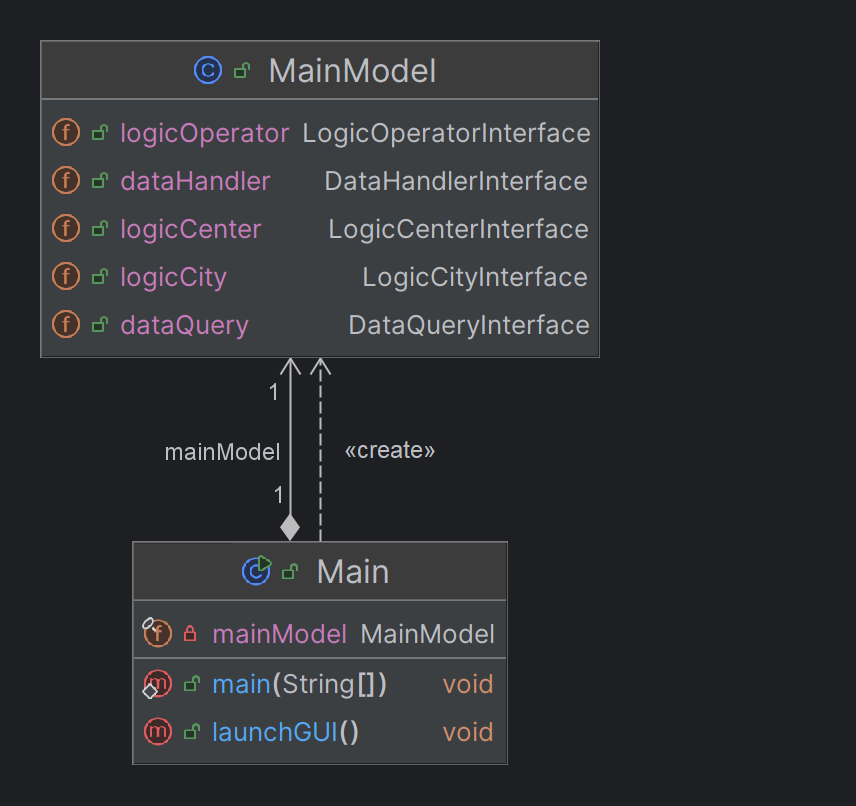
\includegraphics[width=0.7\textwidth]{img/mainModelUML.png}
    \caption{UML della classe MainModel}
    \label{fig:UMLMainModel}
\end{figure}
Oltre aigli attributi è presente solo un costruttore:
\begin{itemize}
    \item \texttt{public MainModel()}: ottiene il registro RMI creato dal server e cerca le interfacce remote necessarie per la comunicazione con lo stesso.
\end{itemize}

\subsection{Package GUI}
In questa sezione verranno descritti il package \texttt{GUI} e le classi che lo compongono.\\

\begin{figure}[H]
    \centering
    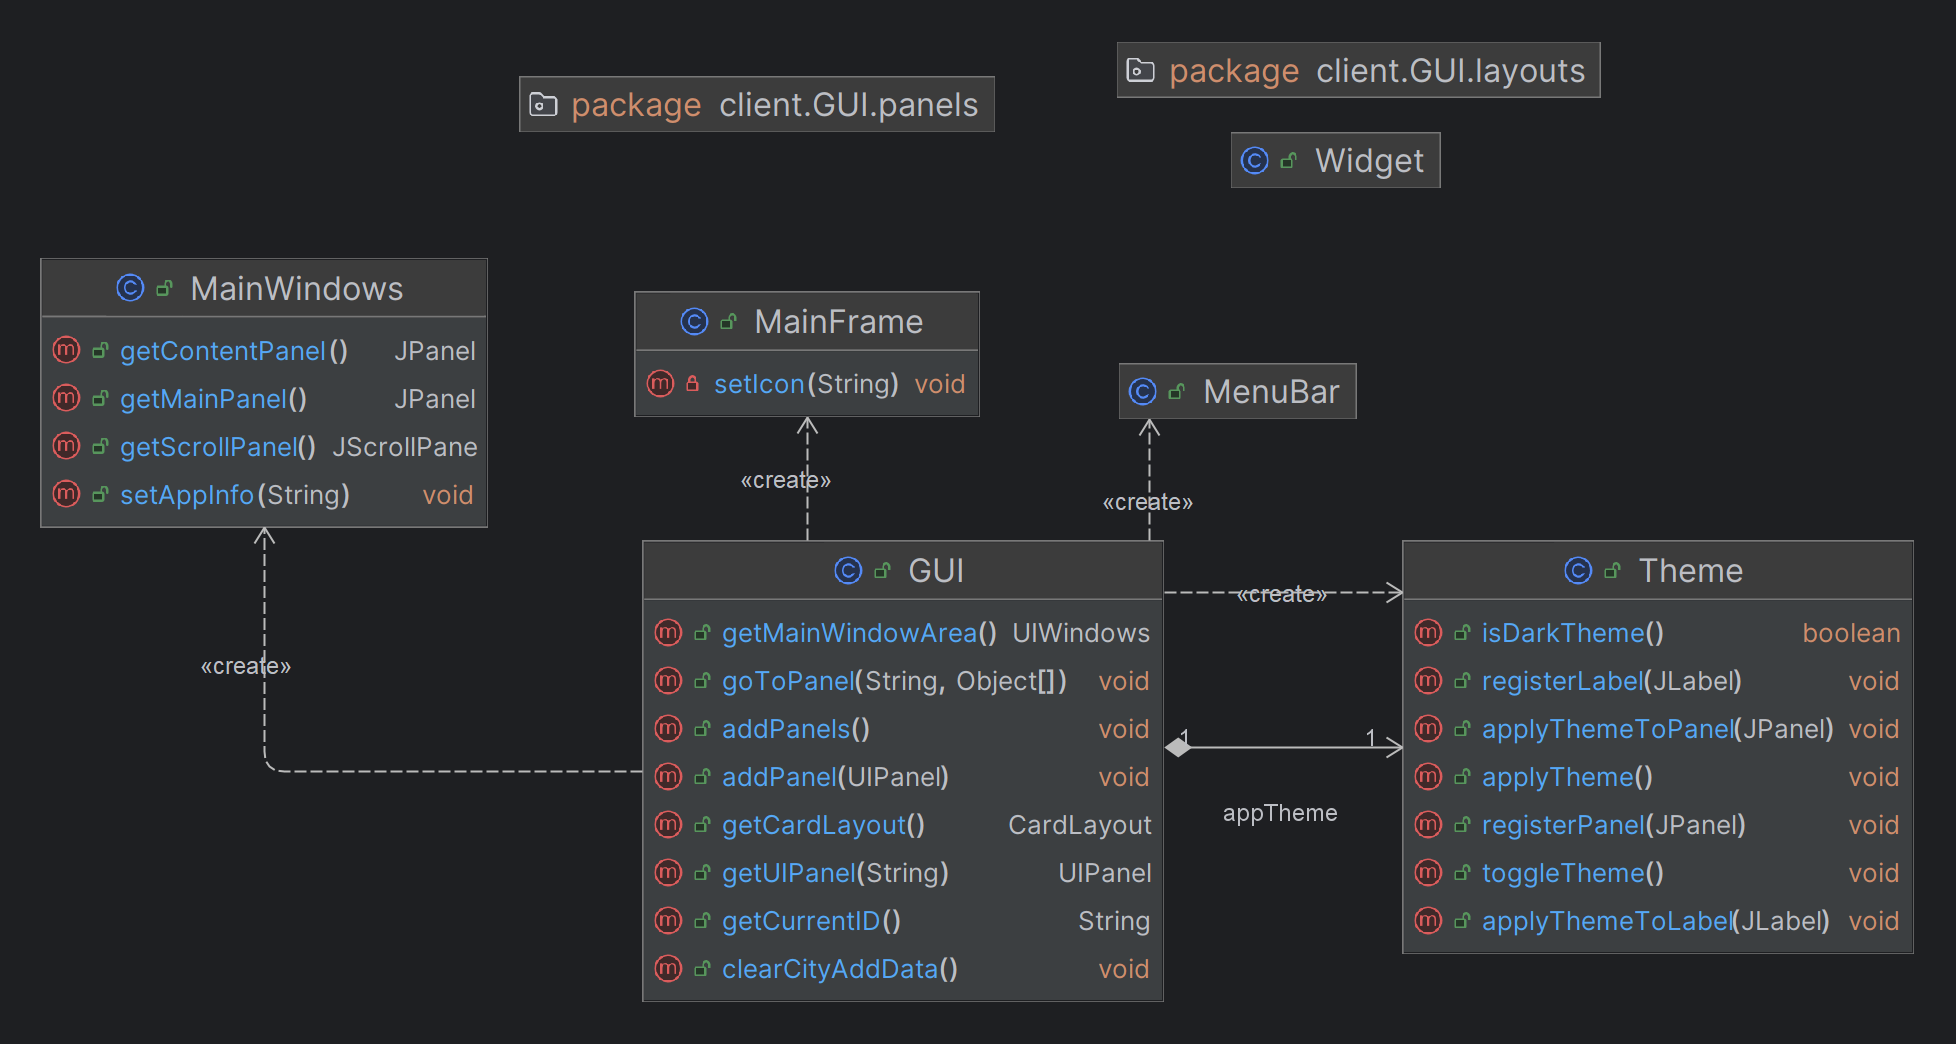
\includegraphics[width=0.9\textwidth]{img/guiPackage.png}
    \caption{UML del package GUI}
    \label{fig:UMLGUI} 
\end{figure}

\subsubsection {GUI}
La classe \texttt{GUI} gestisce l'interfaccia utente dell'applicazione e la navigazione tra diversi pannelli. 
È una componente chiave dell'architettura dell'applicazione, responsabile della creazione e gestione dei pannelli dell'interfaccia utente e della loro visualizzazione.
I metodi di tale classe sono:
\begin{itemize}
    \item \texttt{public void addPanels()}: aggiunge tutti i pannelli utilizzati nell'applicazione.
    \item \texttt{public void addPanel(Interfaces.UIPanel Panel)}: aggiunge un pannello alla mappa dei pannelli e gli applica il tema grafico.
    \item \texttt{public void clearCityAddData()}: pulisce i dati inseriti nel pannello di aggiunta dati di una città.
    \item \texttt{public Interfaces.UIPanel getUIPanel(String ID)}: ottiene un pannello dell'interfaccia utente in base al suo ID.
    \item \texttt{public Interfaces.UIWindows getMainWindowArea()}: restituisce l'area principale dell'applicazione.
    \item \texttt{public CardLayout getCardLayout()}: restituisce il layout a schede utilizzato per la navigazione tra i pannelli.
    \item \texttt{public String getCurrentID()}: restituisce l'ID del pannello corrente.
    \item \texttt{public void goToPanel(String ID, Object[] args)}: cambia il pannello corrente in base all'ID specificato.
\end{itemize}

\subsubsection {Theme}
La classe \texttt{Theme} gestisce il tema grafico dell'applicazione, inclusa la modalitàchiaro/scuro, e applica il tema alle etichette ({@code JLabel}) e ai pannelli ({@code JPanel}).
La classe consente di passare tra modalità chiara e scura e applica automaticamente il tema corrente a tutti i componenti registrati.
I metodi di tale classe sono:
\begin{itemize}
    \item \texttt{public void toggleTheme()}: passa tra modalità chiara e scura.
    \item \texttt{public boolean isDarkTheme()}: controlla se il tema corrente è scuro.
    \item \texttt{public void registerLabel(JLabel label)}: registra un'etichetta per applicare il tema corrente.
    \item \texttt{public void registerPanel(JPanel panel)}: registra un pannello per applicare il tema corrente.
    \item \texttt{public void applyTheme()}: applica il tema corrente a tutti i componenti registrati.
    \item \texttt{public void applyThemeToPanel(JPanel panel)}: applica il tema corrente a un pannello.
    \item \texttt{public void applyThemeToLabel(JLabel label)}: applica il tema corrente a un'etichetta.
\end{itemize}

\subsubsection {Widget}
La classe \texttt{Widget} fornisce componenti grafici comuni utilizzati nell'interfaccia utente dell'applicazione tramite classi interne.\\
Include pannelli di formattazione, pulsanti con cursori personalizzati, etichette per immagini e oggetti per elementi di una lista a discesa. 
Questi componenti sono progettati per facilitare la creazione di interfacce utente coerenti e ben stilizzate.

\begin{figure}[H]
    \centering
    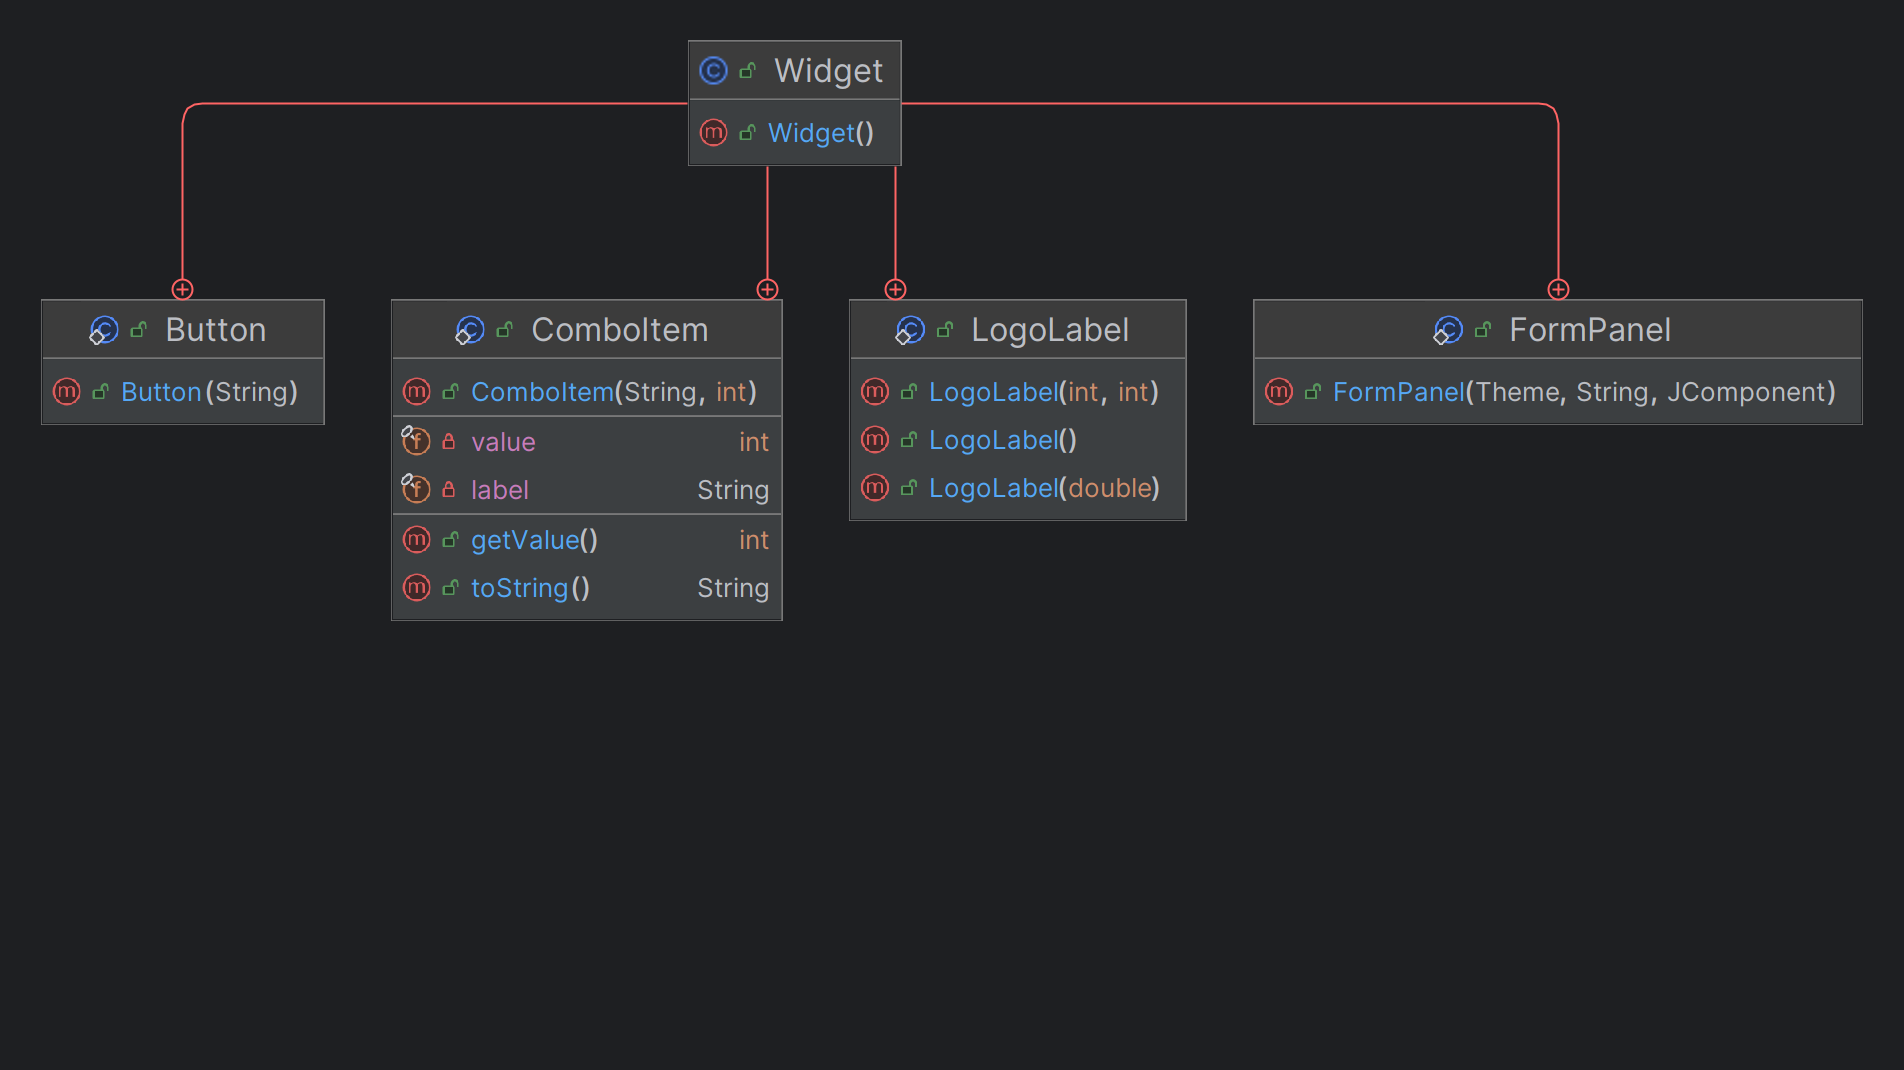
\includegraphics[width=0.9\textwidth]{img/UMLWidget.png}
    \caption{UML della classe Widget}
    \label{fig:UMLWidget}
\end{figure}
I costruttori e metodi delle classi interne sono:
\begin{itemize}
    \item \texttt{public FromPanel(Theme appTheme, String labelText, JComponent activeArea)}: costruttore del pannello di formattazione personalizzato.
    \item \texttt{public Button(String text)}: costruttore di un pulsante con il testo specificato.
    \item \texttt{public LogoLabel()}: crea un'etichetta con le dimensioni predefinite.
    \item \texttt{public LogoLabel(double scale)}: crea un'etichetta con le dimensioni specificate per il logo.
    \item \texttt{public LogoLabel(int width, int height)}: crea un'etichetta dimensioni personalizzate.
    \item \texttt{public ComboItem(String label, int value)}: costruttore di un oggetto per un elemento di una lista a discesa con un'etichetta e un valore associato.
    \item \texttt{public int getValue()}: restituisce il valore associato all'elemento della lista a discesa.
    \item \texttt{public String toString()}: restituisce l'etichetta dell'elemento della lista a discesa.
\end{itemize}

\subsubsection{Package layouts}
In questo package sono presenti le classi che definiscono i layout utilizzati nell'interfaccia grafica dell'applicazione.

\begin{figure}[H]
    \centering
    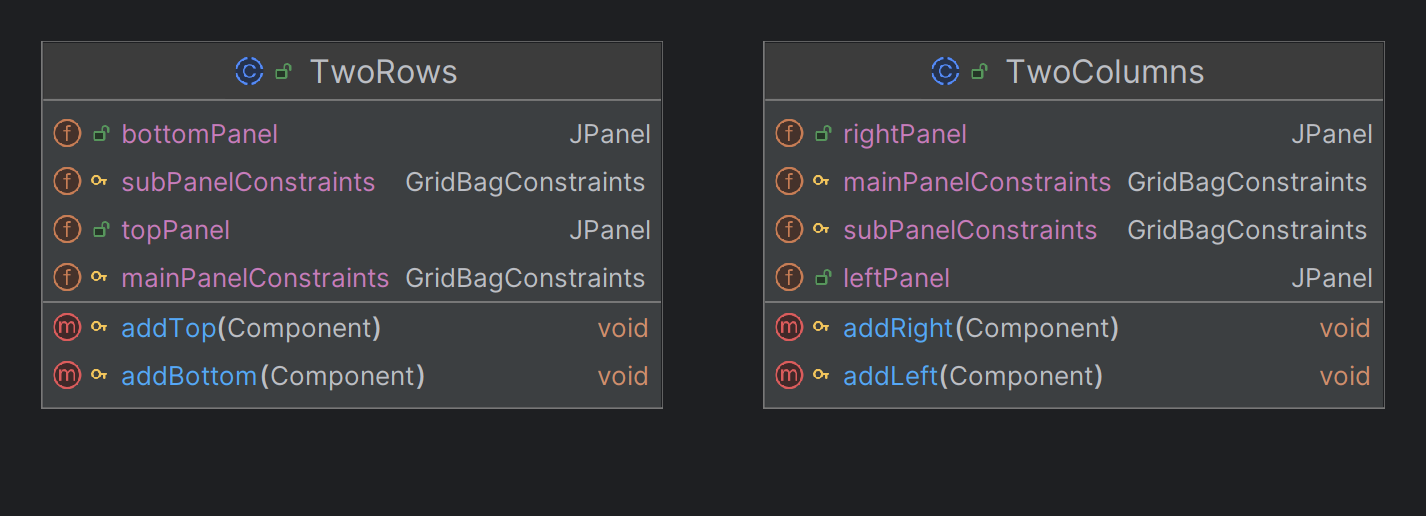
\includegraphics[width=0.9\textwidth]{img/layoutsPackage.png}
    \caption{UML del package layouts}
    \label{fig:UMLLayouts}
\end{figure}
\paragraph{TwoColumns}
La classe astratta \texttt{TwoColumns} rappresenta un layout a due colonne, con un pannello sinistro e un pannello destro. È progettata per essere estesa da altre classi che necessitano di questo tipo di layout.
Entrambi i pannelli utilizzano un \texttt{GridBagLayout} per permettere un layout flessibile dei componenti.
La classe fornisce metodi protetti per aggiungere componenti ai pannelli sinistro e destro.\\
I metodi di tale classe sono:
\begin{itemize}
    \item \texttt{protected void addLeft(Component component)}: aggiunge un componente al pannello sinistro.
    \item \texttt{protected void addRight(Component component)}: aggiunge un componente al pannello destro.
\end{itemize}

\paragraph{TwoRows}
La classe astratta \texttt{TwoRows} rappresenta un layout a due righe per un'interfaccia grafica Swing.
Le due righe contengono un pannello superiore e un pannello inferiore per organizzare i componenti dell'interfaccia.\\
I metodi di tale classe sono:
\begin{itemize}
    \item \texttt{protected void addTop(Component component)}: aggiunge un componente al pannello superiore.
    \item \texttt{protected void addBottom(Component component)}: aggiunge un componente al pannello inferiore.
\end{itemize}

\subsubsection {Package mainElements}
In questo package sono presenti le classi che definiscono gli elementi della finestra principale dell'applicazione.

\begin{figure}[H]
    \centering
    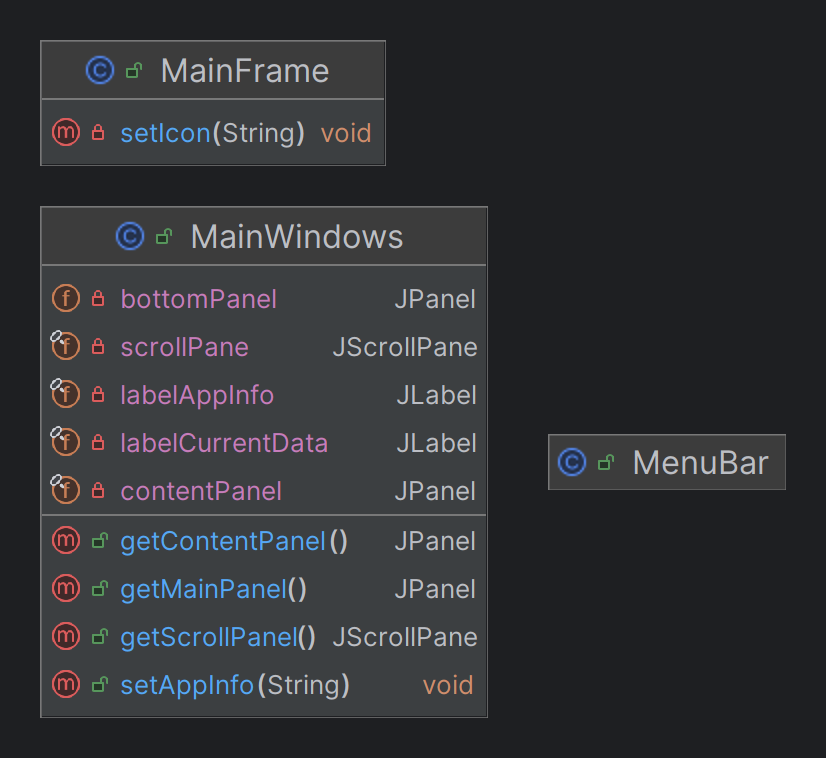
\includegraphics[width=0.6\textwidth]{img/mainElementsPackage.png}
    \caption{UML del package mainElements}
    \label{fig:UMLMainElements}
\end{figure}

\paragraph{MainFrame}
La classe \texttt{MainFrame} rappresenta il frame principale dell'applicazione.
Il frame contiene i componenti principali dell'interfaccia utente e funge da contenitore principale per tutti i widget e pannelli dell'applicazione.
I costruttori e metodi di tale classe sono:
\begin{itemize}
    \item \texttt{public MainFrame()}: configura il frame principale dell'applicazione.
    \item \texttt{private void setIcon(String iconPath)}: imposta l'icona del frame.
\end{itemize}

\paragraph{MainWindows}
La classe \texttt{MainWindows} rappresenta la finestra principale dell'applicazione.
Questa finestra contiene un pannello scorrevole con un layout a schede, in cui vengono visualizzate diverse schermate dell'applicazione. 
Inoltre, nella parte inferiore della finestra, vengono visualizzate informazioni sull'operatore attualmente loggato e l'orario corrente.
I costruttori e metodi di tale classe sono:
\begin{itemize}
    \item \texttt{public MainWindows(CardLayout cardLayout)}: inizializza la finestra principale dell'applicazione impostando il pannello a scorrimento, il layout a schede e aggiungendo timer e informazioni sull'operatore nella parte inferiore della finestra.
    \item \texttt{public JPanel getMainPanel()}: restituisce il pannello principale della finestra.
    \item \texttt{public JScrollPane getScrollPanel()}: restituisce il pannello scorrevole della finestra.
    \item \texttt{public JPanel getContentPanel()}: restituisce il pannello contenente i pannelli a schede.
    \item \texttt{public void setAppInfo(String text)}: imposta le informazioni sull'operatore attualmente loggato.
\end{itemize}

\paragraph{MenuBar}

La classe \texttt{MenuBar} rappresenta la barra del menù dell'interfaccia grafica dell'applicazione.
Questa barra del menù consente la navigazione tra diverse sezioni dell'applicazione e fornisce opzioni per cambiare il tema dell'interfaccia utente e gestire la sessione dell'operatore.
Gli elementi principali del menù includono home, ricerca città, e un sotto-menù per l'area operatore con le opzioni di login, registrazione, gestione città e logout.
All'interno è presente solo il costruttore:
\begin{itemize}
    \item \texttt{public MenuBar(GUI gui)}: imposta il layout della barra del menu, aggiunge gli elementi del menu e gestisce gli eventi di selezione del menu.
\end{itemize}

\subsubsection {Package panels}
In questo package sono presenti le classi che definiscono i pannelli dell'interfaccia grafica dell'applicazione.

\begin{figure}[H]
    \centering
    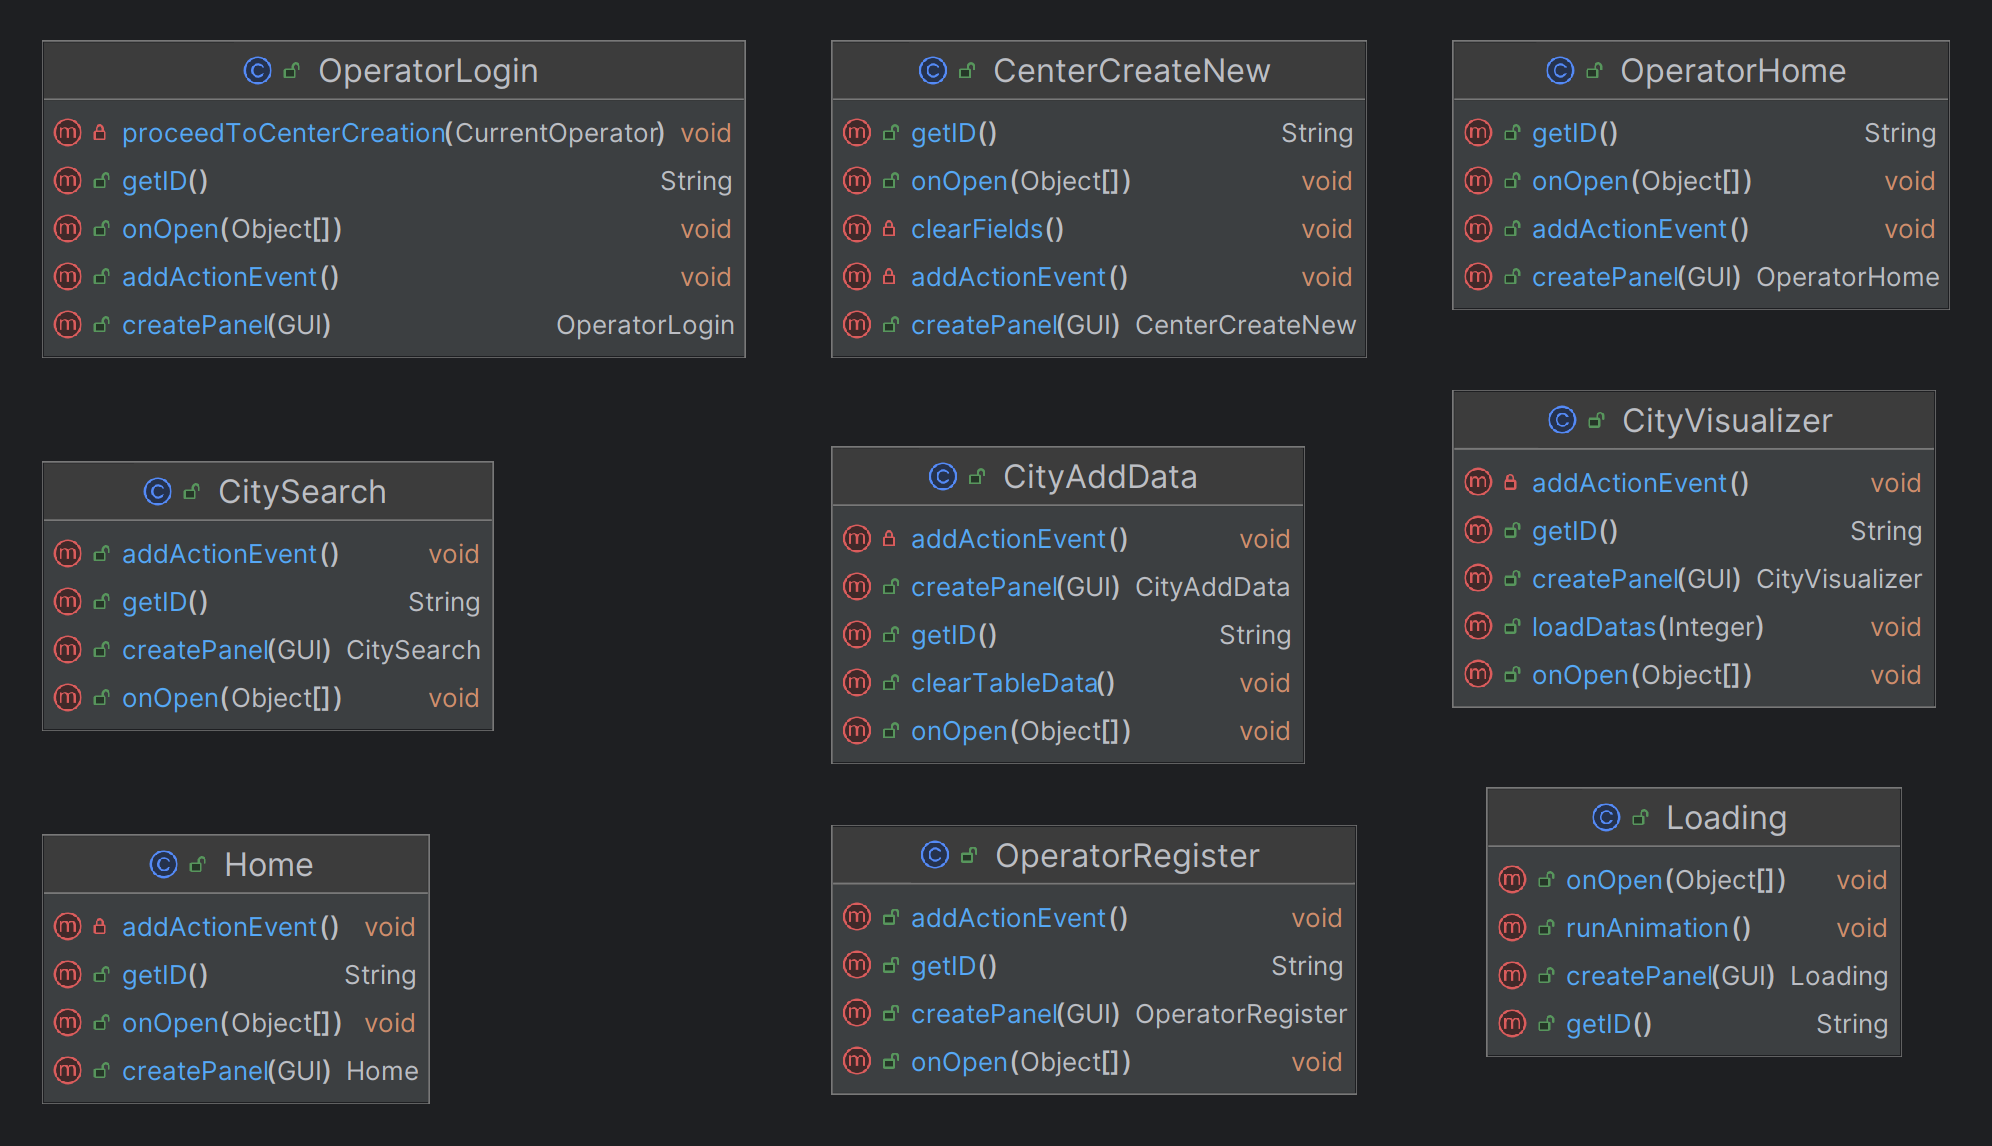
\includegraphics[width=0.9\textwidth]{img/panelsPackage.png}
    \caption{UML del package panels}
    \label{fig:UMLPanels}    
\end{figure}

\paragraph{Loading}
La classe \texttt{Loading} rappresenta un pannello di caricamento animato che viene visualizzato all'avvio dell'applicazione.
Questo pannello mostra il nome dell'applicazione con una serie di punti che si muovono per simulare un caricamento. 
L'animazione prosegue fino a quando il pannello non reindirizza automaticamente all'homepage dell'applicazione.
I metodi di tale classe sono:
\begin{itemize}
    \item \texttt{public void runAnimation()}: avvia l'animazione di caricamento.
    \item \texttt{public Loading createPanel(GUI gui)}: crea il pannello di caricamento.
    \item \texttt{public String getID()}: restituisce l'ID del pannello.
    \item \texttt{public void onOpen(Object[] args)}; gestisce l'apertura del pannello.
\end{itemize}

\paragraph{Home}
La classe \texttt{Home} rappresenta il pannello principale dell'applicazione visualizzato dopo il caricamento iniziale.
Questo pannello fornisce all'utente due opzioni principali: \textbf{Cerca e visualizza dati} per accedere alla funzionalità di ricerca e visualizzazione dei dati, e \textbf{Gestisci area operatore} per accedere alla gestione dell'area riservata agli operatori.
L'utente può selezionare una delle opzioni per avviare le funzionalità specifiche dell'applicazione.
I metodi di tale classe sono:
\begin{itemize}
    \item \texttt{private void addActionEvent()}: aggiunge gli eventi per la navigazione tra i pannelli.
    \item \texttt{public Home createPanel(GUI gui)}: crea il pannello home.
    \item \texttt{public String getID()}: restituisce l'ID del pannello.
    \item \texttt{public void onOpen(Object[] args)}: gestisce l'apertura del pannello.
\end{itemize}

\paragraph{CitySearch}
La classe \texttt{CitySearch} rappresenta il pannello  per effettuare ricerche sulla base di dati delle città.
Gli utenti possono cercare una città per nome o per coordinate geografiche utilizzando i campi di input e i pulsanti forniti.
I metodi di tale classe sono:
\begin{itemize}
    \item \texttt{public void addActionEvent()}: aggiunge gli eventi per la ricerca delle città in base al pulsante premuto.
    \item \texttt{public CitySerch createPanel(GUI gui)}: crea il pannello di ricerca città.
    \item \texttt{public String getID()}: restituisce l'ID del pannello.
    \item \texttt{public void onOpen(Object[] args)}: gestisce l'apertura del pannello.
\end{itemize}

\paragraph{CityVisualizer}

La classe \texttt{CityVisualizer} rappresenta il pannello per la visualizzazione dei dati di una città, inclusi i dati meteorologici relativi a diverse categorie.
È utilizzato nell'applicazione per mostrare dettagli sulla città selezionata e i dati meteorologici associati.
I metodi di tale classe sono:
\begin{itemize}
    \item \texttt{private void addActionEvent()}: aggiunge gli eventi al pulsante per tornare alla schermata precedente.
    \item \texttt{public void loadDatas(Integer cityID)}: carica i dati della città selezionata.
    \item \texttt{public CityVisualizer createPanel(GUI gui)}: crea il pannello di visualizzazione dei dati della città.
    \item \texttt{public String getID()}: restituisce l'ID del pannello.
    \item \texttt{public void onOpen(Object[] args)}: gestisce l'apertura del pannello.
\end{itemize}
Sono presenti anche due classi interne:
\begin{itemize}
    \item \texttt{ToolttipCellRenderer}: classe interna che gestisce il rendering delle celle della tabella.
    \item \texttt{NonEditableCellEditor}: classe interna per l'editor delle celle non modificabili.
\end{itemize}

\begin{figure}[H]
    \centering
    \includegraphics[width=0.9\textwidth]{img/cityVisualizerUML.png}
    \caption{UML della classe CityVisualizer}
    \label{fig:UMLCityVisualizer}
\end{figure}

I metodi di tali classi interne sono:
\begin{itemize}
    \item \texttt{public Component getTableCellRendererComponent(JTable table, Object value, boolean isSelected, boolean hasFocus, int row, int column)}: restituisce il componente per il rendering delle celle della tabella.
    \item \texttt{public boolean isCellEditable(EventObject e)}: restituisce \texttt{false} per indicare che la cella non è modificabile.
\end{itemize}

\paragraph{OperatorHome}
La classe \texttt{OperatorHome} rappresenta il pannello principale per gli operatori dell'applicazione.
Da questo pannello, gli operatori possono scegliere di registrarsi o accedere all'applicazione. 
Questa classe gestisce la navigazione tra il pannello di registrazione e quello di login tramite i pulsanti corrispondenti.
I metodi di tale classe sono:
\begin{itemize}
    \item \texttt{public void addActionEvent()}: aggiunge gli eventi per la navigazione tra i pannelli in base al pulsante premuto.
    \item \texttt{public String getID()}: restituisce l'ID del pannello.
    \item \texttt{public void onOpen(Object[] args)}: gestisce l'apertura del pannello.
\end{itemize}

\paragraph{OperatorRegister}
La classe \texttt{OperatorRegister} rappresenta il pannello utilizzato per la registrazione di un operatore all'interno dell'applicazione.
Questo pannello consente agli operatori di inserire i loro dati personali, come nome, codice fiscale, email, username e password, al fine di creare un nuovo account operatore.
Utilizza il modulo server RMI per la registrazione e gestisce le eccezioni che possono derivare dalla connessione al server o dalle operazioni sul database.
I metodi di tale classe sono:
\begin{itemize}
    \item \texttt{public void addActionEvent()}: aggiunge gli eventi per la registrazione dell'operatore.
    \item \texttt{public OperatorRegister createPanel(GUI gui)}: crea il pannello di registrazione operatore.
    \item \texttt{public String getID()}: restituisce l'ID del pannello.
    \item \texttt{public void onOpen(Object[] args)}: gestisce l'apertura del pannello.
\end{itemize}

\paragraph{OperatorLogin}
La classe \texttt{OperatorLogin} rappresenta il pannello di login per gli operatori dell'applicazione.
Gli operatori possono inserire il loro username e la password per accedere all'applicazione. 
Utilizza un modulo server RMI per autenticare l'operatore e interagisce con un database per recuperare e gestire i dati necessari.
I metodi di tale classe sono:
\begin{itemize}
    \item \texttt{public void addActionEvent()}: aggiunge gli eventi per il login dell'operatore.
    \item \texttt{public OperatorLogin createPanel(GUI gui)}: crea il pannello di login operatore.
    \item \texttt{public String getID()}: restituisce l'ID del pannello.
    \item \texttt{public void onOpen(Object[] args)}: gestisce l'apertura del pannello.
    \item \texttt{private void proceedToCenterCreation(CurrentOperator currentOperator)}: metodo privato che gestisce la creazione o associazione di un centro per l'operatore che ha effettuato il login per la prima volta.

\end{itemize}

\paragraph{CenterCreateNew}
La classe \texttt{CenterCreateNew} rappresenta il pannello per la creazione di un nuovo centro di monitoraggio da parte dell'operatore.
Il pannello consente all'operatore di inserire informazioni sul centro, come il nome, la via, il numero civico, il CAP, il comune, la provincia e le città associate al centro.\\
Una volta inseriti i dati, l'operatore può salvare il centro nel sistema utilizzando i servizi offerti dal modulo server RMI e interagendo con il database.\\
La classe gestisce la validazione dei dati inseriti e fornisce feedback all'operatore in caso di errori.\\
La comunicazione con il server RMI è gestita attraverso l'interfaccia \texttt{DataQueryImp} per le query sui dati e \texttt{MainModel} per la logica di applicazione.
I metodi di tale classe sono:
\begin{itemize}
    \item \texttt{private void clearFields()}: pulisce i campi di input del pannello.
    \item \texttt{private void addActionEvent()}: aggiunge gli eventi per la creazione di un nuovo centro.
    \item \texttt{public CenterCreateNew createPanel(GUI gui)}: crea il pannello di creazione di un nuovo centro.
    \item \texttt{public String getID()}: restituisce l'ID del pannello.
    \item \texttt{public void onOpen(Object[] args)}: gestisce l'apertura del pannello.
\end{itemize}

\paragraph{CityAddData}
La classe \texttt{CityAddData} rappresenta il pannello per l'aggiunta di dati di una città da parte dell'operatore.\\
Il pannello consente all'operatore di inserire i dati relativi alla città selezionata quali: data di rilevamento dati, punteggi per le varie categorie ed eventualmente dei commenti che li descrivono.\\
La classe gestisce la validazione della data inserita, il limite di caratteri per i commenti dei dati e la funzionalità per il salvataggio dei dati inseriti. 
I metodi di tale classe sono:
\begin{itemize}
    \item \texttt{public void clearTableData()}: pulisce i dati inseriti nella tabella.
    \item \texttt{private void addActionEvent()}: aggiunge gli eventi per l'aggiunta dei dati della città.
    \item \texttt{public CityAddData createPanel(GUI gui)}: crea il pannello di aggiunta dati di una città.
    \item \texttt{public String getID()}: restituisce l'ID del pannello.
    \item \texttt{public void onOpen(Object[] args)}: gestisce l'apertura del pannello.
\end{itemize}
Anche in questo caso sono presenti delle classi interne:
\begin{itemize}
    \item \texttt{IntegerCellEditor}: classe interna per l'editor delle celle numeriche.
    \item \texttt{ToolttipCellRenderer}: classe interna che gestisce il rendering delle celle della tabella.
    \item \texttt{NonEditableCellEditor}: classe interna per l'editor delle celle non modificabili.
\end{itemize}
I metodi di tali classi interne sono:
\begin{itemize}
    \item \texttt{public Integer getCellEditorValue()}: restituisce il valore intero selezionato dall'utente.
    \item \texttt{public Component getTableCellRendererComponent(JTable table, Object value, boolean isSelected, boolean hasFocus, int row, int column)}: restituisce il componente per il rendering delle celle della tabella.
    \item \texttt{public boolean isCellEditable(EventObject e)}: resituisce \texttt{false} per indicare che la cella non è modificabile.
\end{itemize}
\section{Pattern utilizzati}

All’interno della classe \texttt{CurrentOperatore.java} sono stati utilizzati due pattern specifici: il \textbf{Singleton} e \textbf{l’Observer}.\\
Il pattern Singleton è utilizzato per garantire che ci sia una sola istanza della classe \texttt{CurrentOperator} nell'applicazione. La classe ha un costruttore privato e un campo statico \texttt{instance}
che rappresenta l'istanza unica della classe. Il metodo \texttt{getInstance()} restituisce l'istanza esistente se è già stata creata o ne crea una nuova se non esiste ancora.
\begin{figure}[H]
    \centering
    \includegraphics[width=1\textwidth]{../../img/Singleton.png}
    \caption{Costruttore della classe CurrentOperator}
    \label{fig:Singleton}
    
\end{figure}

Questo pattern è stato implementato seguendo questo schema:
\begin{figure}[H]
    \centering
    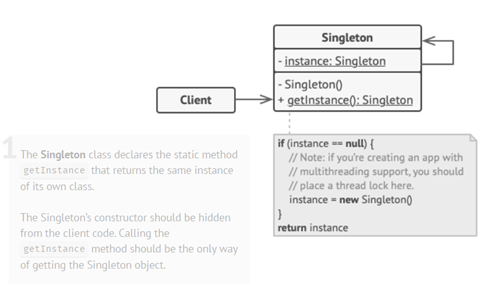
\includegraphics[width=1\textwidth]{../../img/schema_singleton.png}
    \caption{Schema del pattern Singleton}
    \label{fig:SingletonPattern}
    
\end{figure}

Il pattern Observer è utilizzato per notificare altri oggetti quando l'utente corrente cambia. La classe\texttt{CurrentOperator} definisce un'interfaccia \texttt{CurrentUserChangeListener}
che deve essere implementata da tutte le classi interessate ai cambiamenti dell'utente corrente.
\begin{figure}[H]
    \centering
    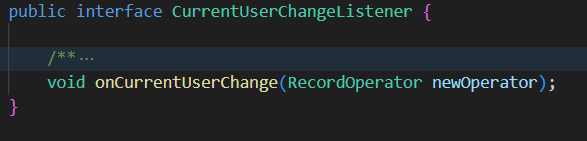
\includegraphics[width=1\textwidth]{../../img/currentUserChangeListener.png}
    \caption{Interfaccia CurrentUserChangeListener}
    \label{fig:Observer 1}
\end{figure}
La classe contiene metodi per aggiungere (\texttt{addCurrentUserChangeListener}) e rimuovere (\texttt{removeCurrentUserChangeListener}) listener interessati ai cambiamenti dell'utente corrente.
Quando l'utente corrente cambia, il metodo \texttt{notifyCurrentUserChange} viene chiamato per notificare tutti i listener registrati.
\begin{figure}[H]
    \centering
    \includegraphics[width=1\textwidth]{../../img/notifyCurrentUserChange.png}
    \caption{Metodo notifyCurrentUserChange}
    \label{fig:Observer 2}
\end{figure}
In questo modo, altre parti dell'applicazione possono essere avvisate quando l'utente corrente cambia, consentendo una gestione flessibile degli eventi correlati all'utente.

Questo pattern è stato implementato seguendo questo schema:
\begin{figure}[H]
    \centering
    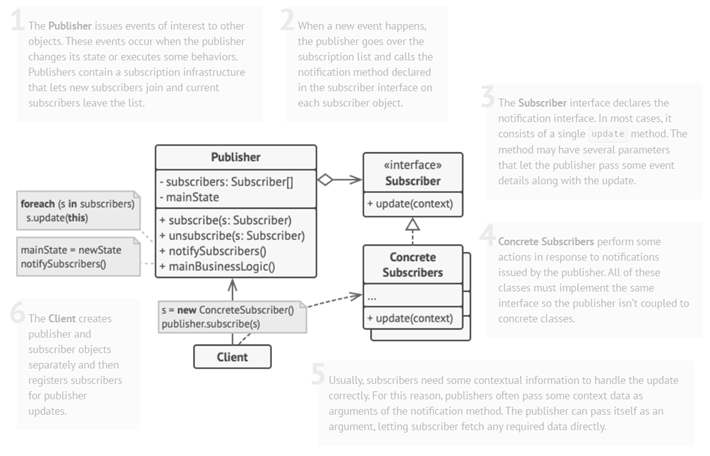
\includegraphics[width=1\textwidth]{../../img/schema_observer.png}
    \caption{Schema del pattern Observer}
    \label{fig:ObserverPattern}
\end{figure}

\end{document}